

\documentclass{article}
\usepackage[utf8]{inputenc}
\usepackage{authblk}
\usepackage{setspace}
\usepackage[margin=1.25in]{geometry}
\usepackage{graphicx}
\graphicspath{{./paper_figures/}}
\usepackage{subcaption}
\usepackage{booktabs}
\usepackage{multirow}
\usepackage[section]{placeins}
\usepackage{amsmath}
\usepackage{lineno}
\linenumbers

%%%%%% Bibliography %%%%%%
% Replace "sample" in the \addbibresource line below with the name of your .bib file.
\usepackage[style=nejm,
citestyle=numeric-comp,
sorting=none]{biblatex}
\addbibresource{sample.bib}

%%%%%% Title %%%%%%
% Full titles can be a maximum of 100 characters, including spaces.
% Title Format: Use title case, capitalizing the first letter of each word, except for certain small words, such as articles and short prepositions
\title{Spectral Preservation in Deep Compression for Hyperspectral Unmixing}

%%%%%% Authors %%%%%%
% Authors should be listed in order of contribution to the paper, by first name, then middle initial (if any), followed by last name.
% Authors should be listed in the order in which they will appear in the published version if the manuscript is accepted.
% Use an asterisk (*) to identify the corresponding author, and be sure to include that person’s e-mail address. Use symbols (in this order: †, ‡, §, ||, ¶, #, ††, ‡‡, etc.) for author notes, such as present addresses, “These authors contributed equally to this work” notations, and similar information.
% You can include group authors, but please include a list of the actual authors (the group members) in the Supplementary Materials.
\author[1*$\dag$]{Author One}
\author[2$\dag$]{Author Two}
\author[2]{Author Three}
\author[1,2]{Author Four}

%%%%%% Affiliations %%%%%%
\affil[1]{Department of Physics, A University, City, Country.}
\affil[2]{Department of Astronomy, B University, City, Country.}
\affil[*]{Address correspondence to: email@email.com}
\affil[$\dag$]{These authors contributed equally to this work.}

%%%%%% Date %%%%%%
% Date is optional
\date{}

%%%%%% Spacing %%%%%%
% Use paragraph spacing of 1.5 or 2 (for double spacing, use command \doublespacing)
\onehalfspacing

\begin{document}

\maketitle

%%%%%% Abstract %%%%%%
\begin{abstract}
The abstract should be a single paragraph written in plain language that a general reader can understand. Do not include citations, figures, tables, or undefined abbreviations in the abstract. Any abbreviations that appear in the title should be defined in the abstract. The length should be 200 words and not exceed 250 words, to include:
\begin{itemize}
    \item An opening sentence that states the question/problem addressed by the research AND
    \item Enough background content to give context to the study AND
    \item A brief statement of primary results AND
    \item A short concluding sentence.
\end{itemize}
\end{abstract}

%%%%%% Main Text %%%%%%



\section{Introduction}

% --- BLOCK 1: Hyperspectral contexto ---
Hyperspectral remote sensing provides detailed spectral measurements of the Earth's surface, enabling the discrimination of materials with similar spatial appearance but distinct spectral responses. Modern hyperspectral sensors acquire hundreds of contiguous spectral bands within the range of 380--2500~nm at resolutions of approximately 5--10~nm, generating rich spectral signatures for every pixel in the scene~\cite{gimenez2025hyperspectral, hong2026hyperspectral}. However, this high spectral resolution also introduces substantial redundancy, since adjacent bands often contain highly correlated information. As a result, hyperspectral datasets present high storage and transmission demands, increased computational complexity, and potential numerical difficulties in subsequent analysis tasks. Consequently, dimensionality reduction has become a fundamental stage in hyperspectral image processing, seeking compact representations that preserve the essential spectral information while reducing data dimensionality. Despite decades of research, achieving efficient compression without compromising the spectral fidelity required by downstream applications remains an active research challenge \cite{vaddi2024}.

% --- BLOCK 2: PCA estandar ---

Traditionally, Principal Component Analysis (PCA) has been the most widely adopted dimensionality reduction technique in hyperspectral image processing due to its simplicity, low computational cost, and ability to achieve substantial compression while retaining most of the data variance~\cite{gimenez2025hyperspectral, hong2026hyperspectral}. However, PCA relies on linear projections and assumes that the underlying spectral structure can be adequately represented in a linear subspace. This assumption limits its ability to model complex nonlinear relationships commonly observed in hyperspectral scenes, such as multiple scattering effects in urban environments and intimate mixtures in heterogeneous soils \cite{gimenez2025hyperspectral, ren2026advances}. These limitations have motivated an increasing interest in deep learning-based dimensionality reduction methods capable of learning richer nonlinear latent representations.

%%%----------------------- Dejarlo arriba para que se plotee bien -----------------------
\begin{figure*}[t]
    \centering
    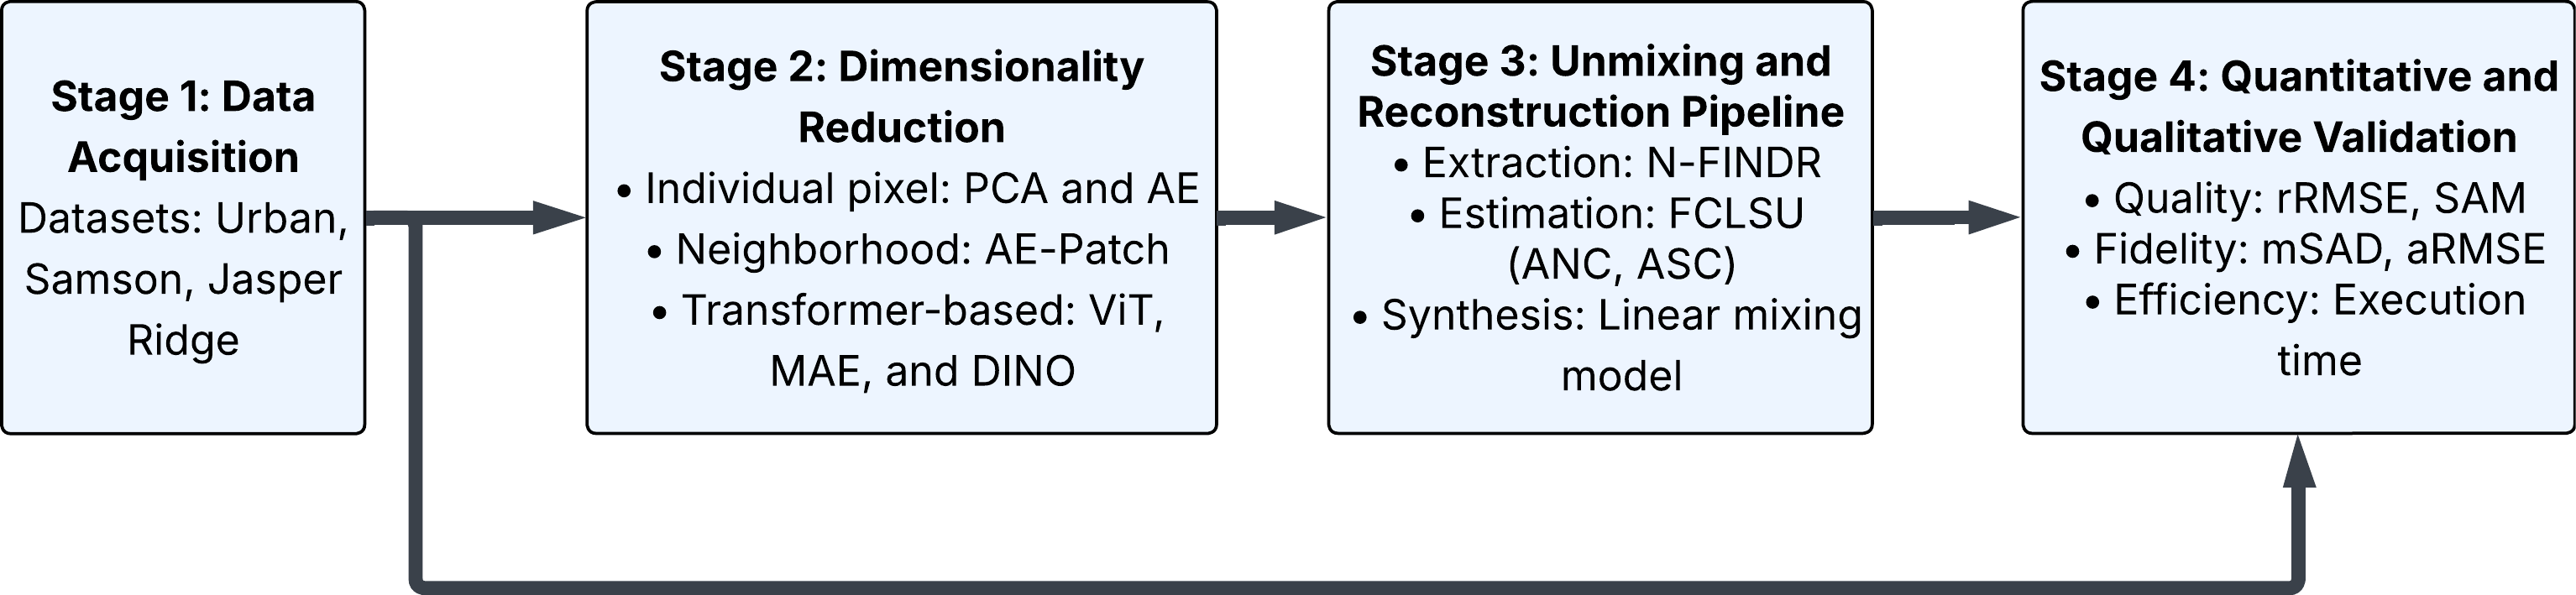
\includegraphics[width=0.85\textwidth]{paper_figures/Met.png}
    \caption{Methodological flow of the proposed framework for dimensionality reduction, linear spectral unmixing, and quantitative validation.}
    \label{fig:flujo_metodologico}
\end{figure*}


Given these limitations, the remote sensing community has progressively adopted deep learning architectures for dimensionality reduction and spectral unmixing. Autoencoders (AE) emerged as one of the first deep learning alternatives to PCA, enabling nonlinear dimensionality reduction through encoder--decoder architectures capable of learning compact latent representations directly from spectral data~\cite{Chen2014, hong2021egunet}. To overcome the lack of spatial context in pixel-wise models, spatial autoencoders (AE-Patch) incorporate information from neighboring pixels, improving the characterization of local spatial-spectral structures and transition regions~\cite{Chen2014, qi2022sscu}. More recently, Vision Transformers (ViT)~\cite{dosovitskiy2021image} introduced self-attention mechanisms that capture long-range spectral and spatial dependencies, extending representation learning beyond local neighborhood interactions~\cite{ghosh2022transformer, Alzubaidi2026S3ViT}; while self-supervised architectures such as Masked Autoencoders (MAE)~\cite{He2022, li2024s2mae} and DINO~\cite{Caron2021} have demonstrated the ability to learn robust latent representations from large amounts of unlabeled data. Despite these advances, the extent to which such representations preserve the spectral information required by downstream hyperspectral analysis tasks remains insufficiently understood.


% --- BLOCK 4: reducido, unminxing ---
% Nevertheless, the ability of these architectures to model complex patterns does not guarantee the preservation of radiometric information at the sub-pixel level. Spectral unmixing requires decomposing each mixed pixel to identify pure materials (endmembers) and estimate their proportions (abundances) under strict non-negativity and sum-to-one constraints~\cite{bioucas2012hyperspectral}, and any distortion introduced during compression propagates and amplifies non-linearly through the inversion stages~\cite{hong2026hyperspectral, ren2026advances}. It is therefore imperative to rigorously evaluate the spectral fidelity limits preserved by these new artificial intelligence-based paradigms.
This question becomes particularly relevant in spectral unmixing, where each pixel must be decomposed into constituent materials and their corresponding abundances under physically meaningful constraints~\cite{bioucas2012hyperspectral}. Because abundance estimation relies directly on the integrity of spectral signatures, distortions introduced during dimensionality reduction may propagate through the inversion process and affect the final unmixing results~\cite{hong2026hyperspectral, ren2026advances}. Consequently, spectral unmixing provides a rigorous framework for evaluating the fidelity of compressed hyperspectral representations.

% --- BLOCK 5: Experimental design (Reducido sin redundar with Sec. 2) ---
% To isolate the effect of the compression stage from downstream processing, we fix the endmember extraction (N-FINDR) and abundance inversion (FCLSU) algorithms across three benchmark datasets of increasing complexity: Samson ($m=3$), Jasper Ridge ($m=4$), and Urban ($m=4$)~\cite{gimenez2025hyperspectral}. This controlled design, detailed in Section~\ref{sec:methodology}, ensures that any observed variation in reconstruction quality ($rRMSE$, $SAM$), abundance accuracy ($aRMSE$), or computational cost is attributable exclusively to the dimensionality reduction method under evaluation.
%To isolate the effect of dimensionality reduction from subsequent processing stages, this study employs a controlled experimental design in which endmember extraction (N-FINDR) and abundance estimation (FCLSU) remain fixed in three reference datasets of increasing complexity: Samson ($m=3$), Jasper Ridge ($m=4$), and Urban ($m=4$)~\cite{gimenez2025hyperspectral}. In this framework, variations in reconstruction quality, abundance estimation accuracy, and computational cost can be attributed exclusively to the compression method under evaluation.


To isolate the effect of dimensionality reduction from subsequent processing stages, this study employs a controlled experimental design in which endmember extraction (N-FINDR) and abundance estimation (FCLSU) remain fixed across three reference datasets of increasing complexity: Samson ($m=3$), Jasper Ridge ($m=4$), and Urban ($m=4$)~\cite{gimenez2025hyperspectral}. These datasets were obtained from~\cite{ozkan2018endnet}.


% --- BLOCK 6: Objetico y alcanze ---
% The objective of this paper is to evaluate the impact of five deep learning algorithms (AE, AE-Patch, ViT, MAE, and DINO) versus PCA for hyperspectral data compression, measuring the accuracy with which material abundances are identified and estimated within a standardized linear spectral unmixing workflow. The scope is strictly delimited to the evaluation of these dimensionality reduction techniques within said workflow, excluding the acquisition of new scenes and nonlinear unmixing models. With this structure, the research aims to provide an analytical reference framework that clarifies whether the geometric abstraction of deep learning respects the fundamental principles of hyperspectral remote sensing.
Consequently, this paper evaluates the impact of five deep learning dimensionality reduction strategies (AE, AE-Patch, ViT, MAE, and DINO) against the traditional PCA baseline within a standardized spectral unmixing workflow. Beyond comparing compression performance, the study investigates how effectively each method preserves the spectral information required for accurate abundance estimation. By providing a controlled and application-oriented evaluation framework, this work seeks to clarify the practical benefits and limitations of modern deep representations for hyperspectral data compression.


\section{Materials and Methods}
\label{sec:methodology}

The methodological framework of this research is structured through a standardized sequential flow for linear spectral unmixing, which is illustrated in Figure~\ref{fig:flujo_metodologico}. This experimental design isolates the impact of dimensionality reduction techniques by keeping the algorithmic stages of extraction and estimation strictly constant. The computational architecture of this process is detailed below:

\textbf{Stage 1: Data Acquisition.} The process begins with the conditioning of three reference hyperspectral datasets (Urban, Samson, and Jasper Ridge). To ensure reproducibility and a rigorous comparison baseline, the official ground truth from the literature is adopted, fixing a priori the exact number of endmembers ($m$). This establishes identical conditions that allow isolating the performance of the compression models.


\textbf{Stage 2: Dimensionality Reduction.} This stage constitutes the core variable of the experimental design. Six architectures spanning three methodological families are evaluated, each offering a distinct inductive bias for spectral-spatial representation learning:

\textit{Principal Component Analysis (PCA)}~\cite{gimenez2025hyperspectral} performs a linear orthogonal projection that maximizes retained variance. It operates on individual pixel vectors of dimension $B$ and serves as the computational baseline due to its closed-form solution and negligible runtime.

\textit{Standard Autoencoder (AE)}~\cite{Chen2014, hong2021egunet} extends PCA into the nonlinear domain through an encoder--decoder architecture that compresses each $B$-dimensional pixel into a latent code of dimension $d \ll B$, capturing nonlinear inter-band correlations that linear projections cannot model.

\textit{Spatial Autoencoder (AE-Patch)}~\cite{Chen2014, qi2022sscu} addresses the lack of spatial context in pixel-wise models by flattening a $3\times3$ neighborhood into a single vector of dimension $9 \times B$, enabling the encoder to jointly learn spectral and local spatial patterns across material boundaries.

\textit{Vision Transformer (ViT)}~\cite{dosovitskiy2021image, ghosh2022transformer} replaces local convolutions with a global self-attention mechanism that models pairwise dependencies among all input tokens simultaneously, capturing long-range spectral and spatial relationships beyond the reach of fixed-kernel architectures.

\textit{Masked Autoencoder (MAE)}~\cite{He2022, li2024s2mae} extends the transformer paradigm with a self-supervised pretext task in which 50\% of the input tokens are randomly masked and the model must reconstruct them, forcing the encoder to learn contextually rich representations rather than trivial identity mappings.

\textit{DINO (Self-Distillation with No Labels)}~\cite{Caron2021} trains a student network to align its representations with a teacher updated via exponential moving average, encouraging semantically invariant embeddings that are structurally resistant to representation collapse.

All transformer-based models (ViT, MAE, and DINO) receive a $3\times3$ spatial block where each pixel retains its $B$ spectral bands as an independent token. For all methods, the dimensionality of the reduced representation is fixed at $d=q-1$, where $q$ is the number of reference endmembers (denoted by $m$ elsewhere in this study). This choice follows the classical N-FINDR formulation, which maximizes the volume of a simplex with $q$ vertices in a $(q-1)$-dimensional space~\cite{remon2013performance}. It is also consistent with previous work applying nonlinear dimensionality reduction before geometric endmember extraction~\cite{nguyen2012hyperspectral}. Using the same output dimensionality across methods enables a common comparison of the representations, while abundance estimation by FCLSU is retained in the original spectral space.

\textbf{Stage 3: Unmixing and Reconstruction Pipeline.} N-FINDR is applied to the reduced representations to identify the $q$ vertices of the endmember simplex and select the corresponding pixels. The original full-spectrum signatures of these pixels are then used to form the endmember matrix. The Fully Constrained Least Squares Unmixing (FCLSU) algorithm estimates fractional abundances by fitting this matrix to the original hyperspectral data, while enforcing abundance non-negativity (ANC) and abundance sum-to-one (ASC). Finally, the endmember matrix and abundance estimates are combined through the linear mixing model to reconstruct the hyperspectral cube. A comprehensive overview of this standard workflow is provided in~\cite{bioucas2012hyperspectral}.


\textbf{Stage 4: Quantitative and Qualitative Validation.} Performance is evaluated by contrasting estimated outputs against ground truth through both quantitative metrics and qualitative spatial analysis~\cite{bioucas2012hyperspectral}.

\textit{Global reconstruction quality} is assessed by two complementary metrics. The reconstruction Root Mean Squared Error (rRMSE) measures the residual between the dataset-normalized cube $\mathbf{X}$ and its reconstruction $\hat{\mathbf{X}}$ over $P$ pixels and $B$ spectral bands~\cite{gimenez2025hyperspectral}:
\begin{equation}
    rRMSE = \sqrt{\frac{1}{PB}\sum_{p=1}^{P}\sum_{b=1}^{B}
    (X_{pb}-\hat{X}_{pb})^2}
    = \frac{\left\| \mathbf{X} - \hat{\mathbf{X}} \right\|_F}{\sqrt{PB}}
    \label{eq:rrmse}
\end{equation}
Here, the prefix $r$ denotes reconstruction, not relative normalization. The
same definition is used for a region of interest by restricting the pixels
to that region. A pixelwise error map applies it across the $B$ bands of
each pixel; regional rRMSE is the root mean square of those pixelwise errors.
The separate abundance metric aRMSE retains its existing definition.
The Spectral Angle Mapper (SAM) measures average angular divergence between corresponding pixel spectra, capturing shape distortions independently of amplitude scaling~\cite{bioucas2012hyperspectral}:
\begin{equation}
    SAM = \frac{1}{P} \sum_{i=1}^{P} \arccos \left( \frac{\mathbf{x}_i^T \hat{\mathbf{x}}_i}{\left\| \mathbf{x}_i \right\| \left\| \hat{\mathbf{x}}_i \right\|} \right)
    \label{eq:sam}
\end{equation}
where $P$ is the total number of pixels and $\mathbf{x}_i$, $\hat{\mathbf{x}}_i$ are the original and reconstructed spectra of the $i$-th pixel.

\textit{Endmember fidelity} is quantified by mean Spectral Angle Distance (mSAD), which averages angular error between each extracted endmember $\mathbf{e}_j$ and its corresponding ground truth reference $\mathbf{e}_j^{*}$~\cite{ghosh2022transformer}:
\begin{equation}
    mSAD = \frac{1}{m} \sum_{j=1}^{m} \arccos \left( \frac{\mathbf{e}_j^T \mathbf{e}_j^{*}}{\left\| \mathbf{e}_j \right\| \left\| \mathbf{e}_j^{*} \right\|} \right)
    \label{eq:msad}
\end{equation}

\textit{Abundance accuracy} is measured by abundance Root Mean Squared Error (aRMSE), computed over all $P$ pixels and $m$ endmembers between the estimated and ground truth abundance matrices~\cite{gimenez2025hyperspectral}.

\textit{Computational efficiency} is measured by total wall-clock execution time per model and dataset, encompassing training, inference, and unmixing~\cite{vaddi2024}.

Visual inspection of spatial rRMSE error maps and estimated abundance maps identifies localized deficiencies—such as error concentration along material boundaries, representation collapse patterns, and class omission—that aggregate metrics alone cannot reveal~\cite{bioucas2012hyperspectral,ozkan2018endnet}.

All experiments were executed on an Ubuntu 24.04 LTS workstation powered by an Intel Core i9-14900KF CPU and an NVIDIA GeForce RTX 5090 GPU (32~GB VRAM).





\section{Results}
\label{sec:results}
This section evaluates the impact of six dimensionality reduction methods on hyperspectral spectral unmixing across three benchmark datasets (Jasper Ridge, Samson, and Urban). The comparison includes a linear baseline (PCA), autoencoder-based models (AE and AE-Patch), and transformer-based architectures (ViT, MAE, and DINO). The analysis focuses on spectral fidelity, computational efficiency, and spatial distribution of reconstruction errors.

\subsection{Global Accuracy and Spectral Fidelity}
\label{subsec:quantitative_analysis}

Figure~\ref{fig:performance_heatmap} shows strongly dataset-dependent reconstruction rankings. In Jasper Ridge, MAE and ViT obtain the lowest rRMSE values (0.0496 and 0.0514), closely followed by PCA (0.0560), whereas DINO records the highest error (0.1116). In Samson, DINO achieves the lowest rRMSE (0.0995), followed by MAE (0.1095), while PCA and AE-Patch produce the largest errors (0.1501 and 0.1482). In Urban, DINO again ranks first (0.1007), with ViT (0.1167) and AE-Patch (0.1204) providing the next best reconstructions; PCA performs worst (0.2894), and AE and MAE also show comparatively high errors. These changes in ranking show that belonging to a transformer-based family does not by itself predict reconstruction performance: DINO moves from the weakest result in Jasper Ridge to the strongest in Samson and Urban, while MAE performs well in Jasper Ridge and Samson but degrades substantially in Urban.

Although these patterns may be compatible with differences in local versus global context modeling, the evaluated architectures also differ in other design and training choices. The present comparison therefore does not isolate the effects of attention, spatial context, or any particular training objective; controlled ablation experiments would be needed to attribute performance differences to these factors.

\begin{figure}[htbp]
    \centering
    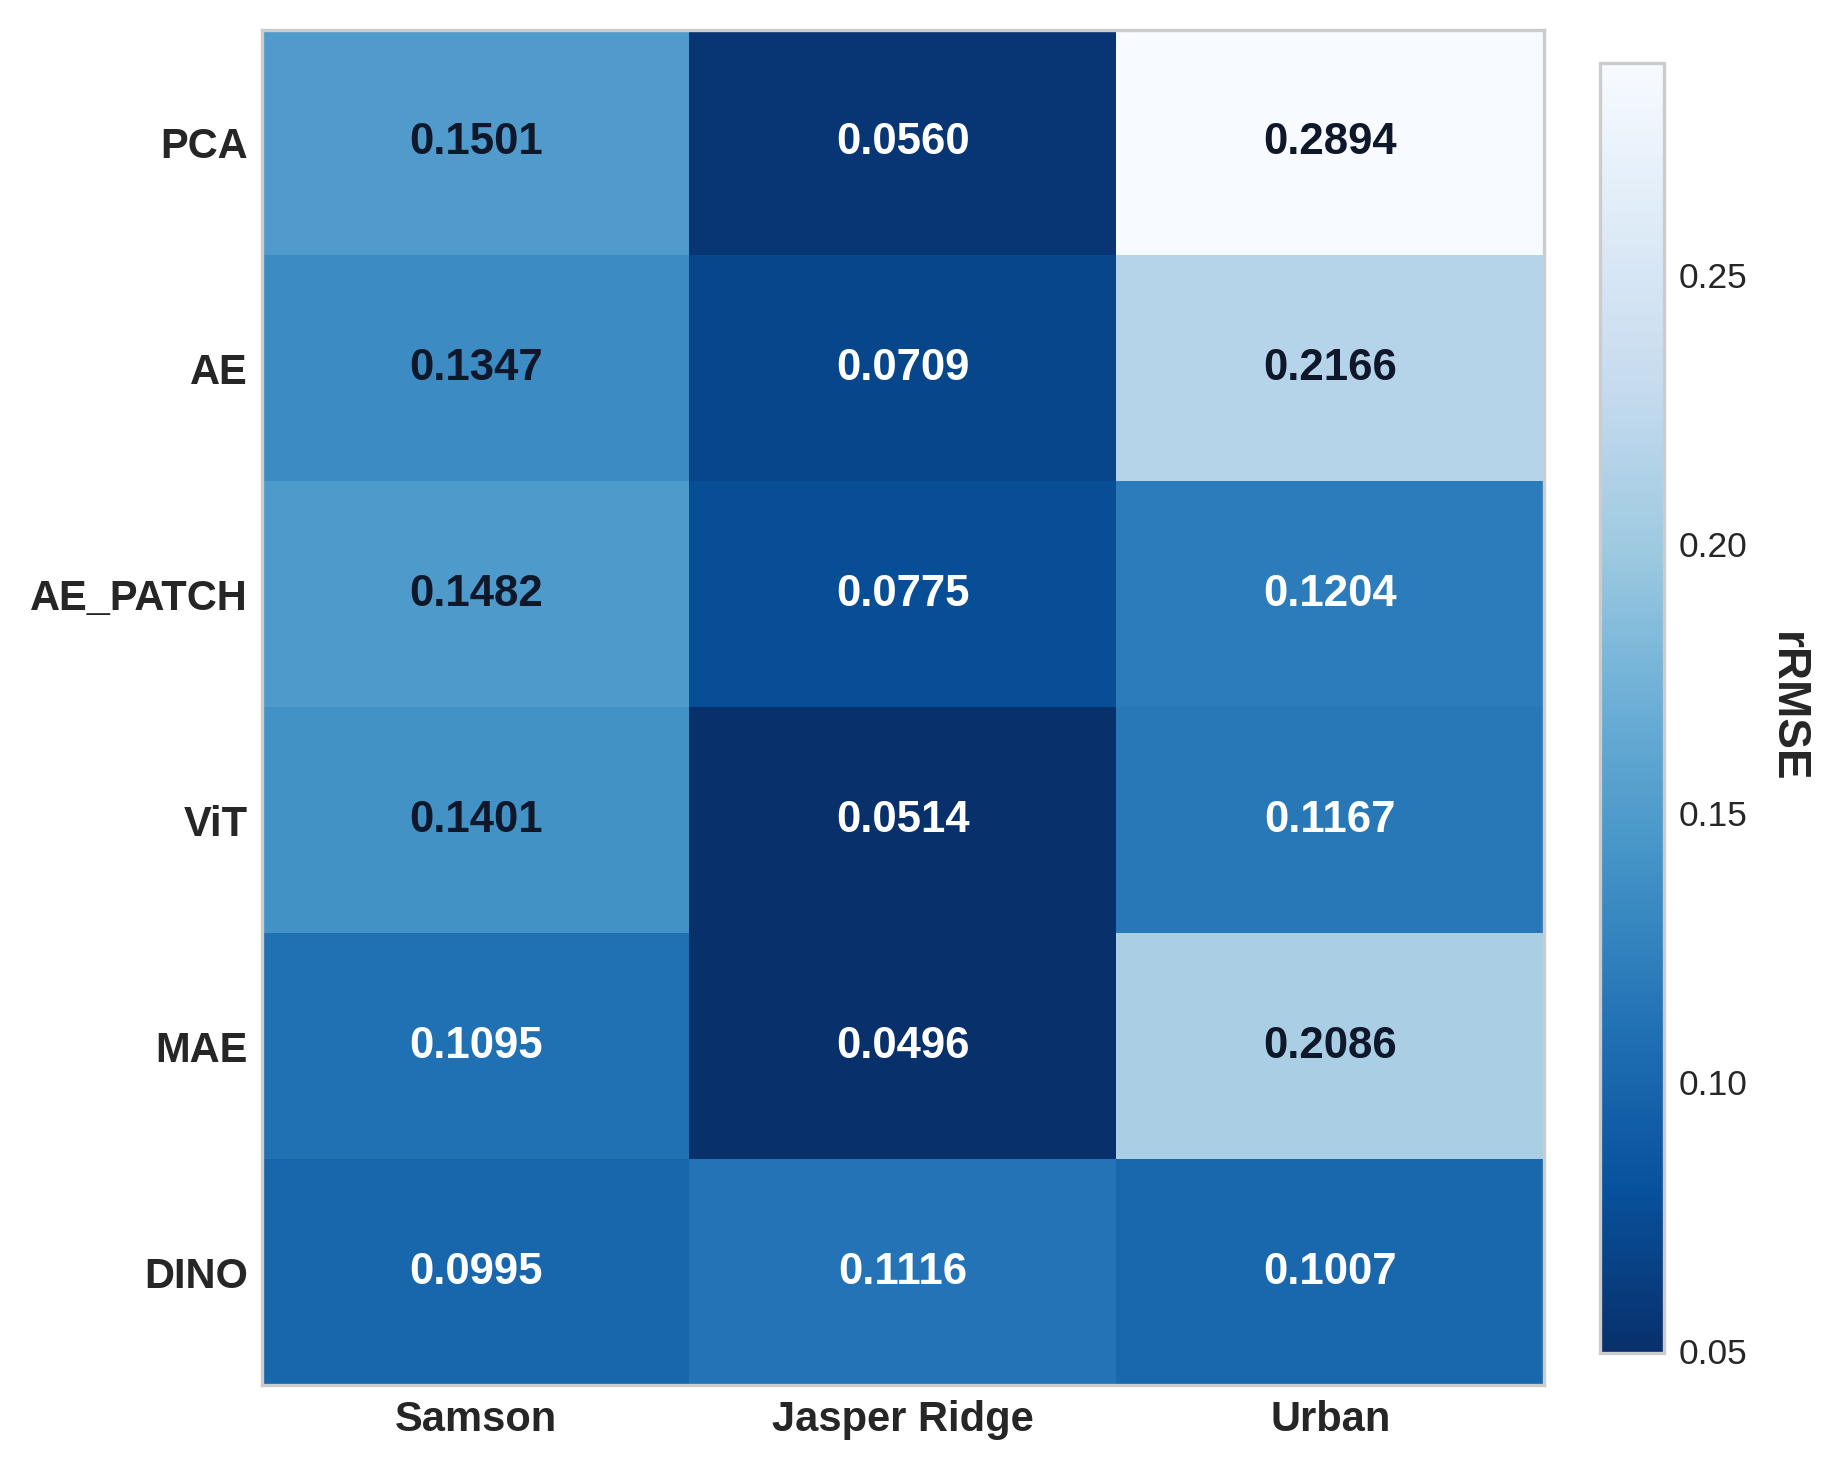
\includegraphics[width=0.75\textwidth]{paper_figures/heatmap_rendimiento.png}
    \caption{Global accuracy heatmap (rRMSE) for the evaluated models.}
    \label{fig:performance_heatmap}
\end{figure}

Regarding physical fidelity, Table~\ref{tab:quantitative_metrics} summarizes the spectral (mSAD), angular (SAM), and abundance estimation (aRMSE) errors obtained across the evaluated datasets. No method or architectural family dominates all datasets and metrics. In Jasper Ridge, MAE achieves the lowest mSAD and aRMSE, whereas ViT obtains the lowest SAM. In Samson, AE-Patch obtains the lowest mSAD, PCA the lowest SAM, and DINO the lowest aRMSE. DINO achieves the best values for all three metrics in Urban, but does not retain this advantage in Jasper Ridge. The results therefore support a dataset- and metric-dependent comparison rather than a uniform advantage for transformer-based representations.

The Urban dataset provides the clearest advantage for DINO, which obtains the lowest mSAD, SAM, and aRMSE in this scene. Other transformer-based models remain competitive in selected measures but do not show the same consistency, and AE-Patch records substantially higher SAM and aRMSE despite its use of local spatial context.

Urban also highlights important differences in model behavior under highly mixed spectral conditions. Within this dataset, DINO combines the strongest quantitative performance with competitive reconstruction accuracy. Nevertheless, the present experimental design does not isolate self-distillation from the other architectural and training differences between models. Consequently, the Urban results demonstrate the effectiveness of the evaluated DINO configuration for this scene, but do not establish self-distillation as the cause of the improvement.

\begin{table}[htbp]
    \centering
    \caption{Quantitative comparison of endmember fidelity (mSAD), cube reconstruction quality (SAM), and abundance estimation accuracy (aRMSE) across the three benchmark datasets.}
    \label{tab:quantitative_metrics}
    \small
    \renewcommand{\arraystretch}{1.15}
    \setlength{\tabcolsep}{3pt}
    \begin{tabular}{l ccc ccc ccc}
        \toprule
        \multirow{2}{*}{\textbf{Method}} & \multicolumn{3}{c}{\textbf{Jasper Ridge}} & \multicolumn{3}{c}{\textbf{Samson}} & \multicolumn{3}{c}{\textbf{Urban}} \\
        \cmidrule(lr){2-4} \cmidrule(lr){5-7} \cmidrule(lr){8-10}
         & \shortstack{\textbf{mSAD}\\($^\circ$)} & \shortstack{\textbf{SAM}\\($^\circ$)} & \textbf{aRMSE} & \shortstack{\textbf{mSAD}\\($^\circ$)} & \shortstack{\textbf{SAM}\\($^\circ$)} & \textbf{aRMSE} & \shortstack{\textbf{mSAD}\\($^\circ$)} & \shortstack{\textbf{SAM}\\($^\circ$)} & \textbf{aRMSE} \\
        \midrule
        PCA       & 9.19          & 8.86          & 0.1187          & 4.02          & \textbf{3.06} & 0.1116          & 25.57         & 7.02          & 0.2543 \\
        AE        & 13.56         & 7.60          & 0.1977          & 3.90          & 3.25          & 0.0935          & 23.47         & 7.68          & 0.2830 \\
        AE-Patch & 21.06         & 11.87         & 0.2108          & \textbf{2.79} & 3.59          & 0.0869          & 16.41         & 17.52         & 0.3855 \\
        ViT       & 7.24          & \textbf{5.71} & 0.0998          & 4.63          & 4.22          & 0.1188          & 20.01         & 7.29          & 0.3336 \\
        MAE       & \textbf{7.08} & 6.02          & \textbf{0.0957} & 4.36          & 3.14          & 0.1087          & 20.21         & 10.10         & 0.2167 \\
        DINO      & 19.72         & 8.03          & 0.3239          & 4.27          & 3.25          & \textbf{0.0695} & \textbf{6.94} & \textbf{4.41} & \textbf{0.1686} \\
        \bottomrule
    \end{tabular}
    \par\smallskip
    \begin{minipage}{\textwidth}
        \footnotesize
        \textit{Note:} mSAD: mean Spectral Angle Distance (endmember extraction error); SAM: Spectral Angle Mapper (global reconstruction error); aRMSE: abundance Root Mean Squared Error. Bold values denote the best result in each column.
    \end{minipage}
\end{table}

The comparison among rRMSE, mSAD, and aRMSE shows that accurate cube reconstruction or endmember identification does not necessarily translate into accurate abundance estimation. In Jasper Ridge, PCA achieves an rRMSE close to those of MAE and ViT but does not lead the endmember or abundance metrics. In Samson, AE-Patch obtains the lowest mSAD but not the lowest rRMSE or aRMSE, whereas DINO achieves the best rRMSE and aRMSE with a higher mSAD. The contrast is especially clear in Urban, where AE-Patch attains the third-lowest rRMSE but records the highest aRMSE and SAM. These discrepancies indicate that abundance inversion can remain a bottleneck even when the compressed cube is reconstructed accurately or endmembers are identified with low spectral error.

\subsection{Computational Efficiency}
\label{subsec:frontera_eficiencia}

Figure~\ref{fig:frontera_eficiencia} illustrates the trade-off between reconstruction accuracy and computational cost of the dimensionality reduction methods evaluated. Transformer-based configurations attain some of the lowest reconstruction errors, particularly in the more complex datasets, but require substantially longer execution times than PCA and conventional autoencoders. At the opposite extreme, PCA offers the highest computational efficiency, while AE and AE-Patch occupy an intermediate position between these regimes. Since accuracy rankings vary by dataset and metric, computational cost should be considered together with the specific fidelity criterion required by the target application.

\begin{figure}[htbp]
    \centering
    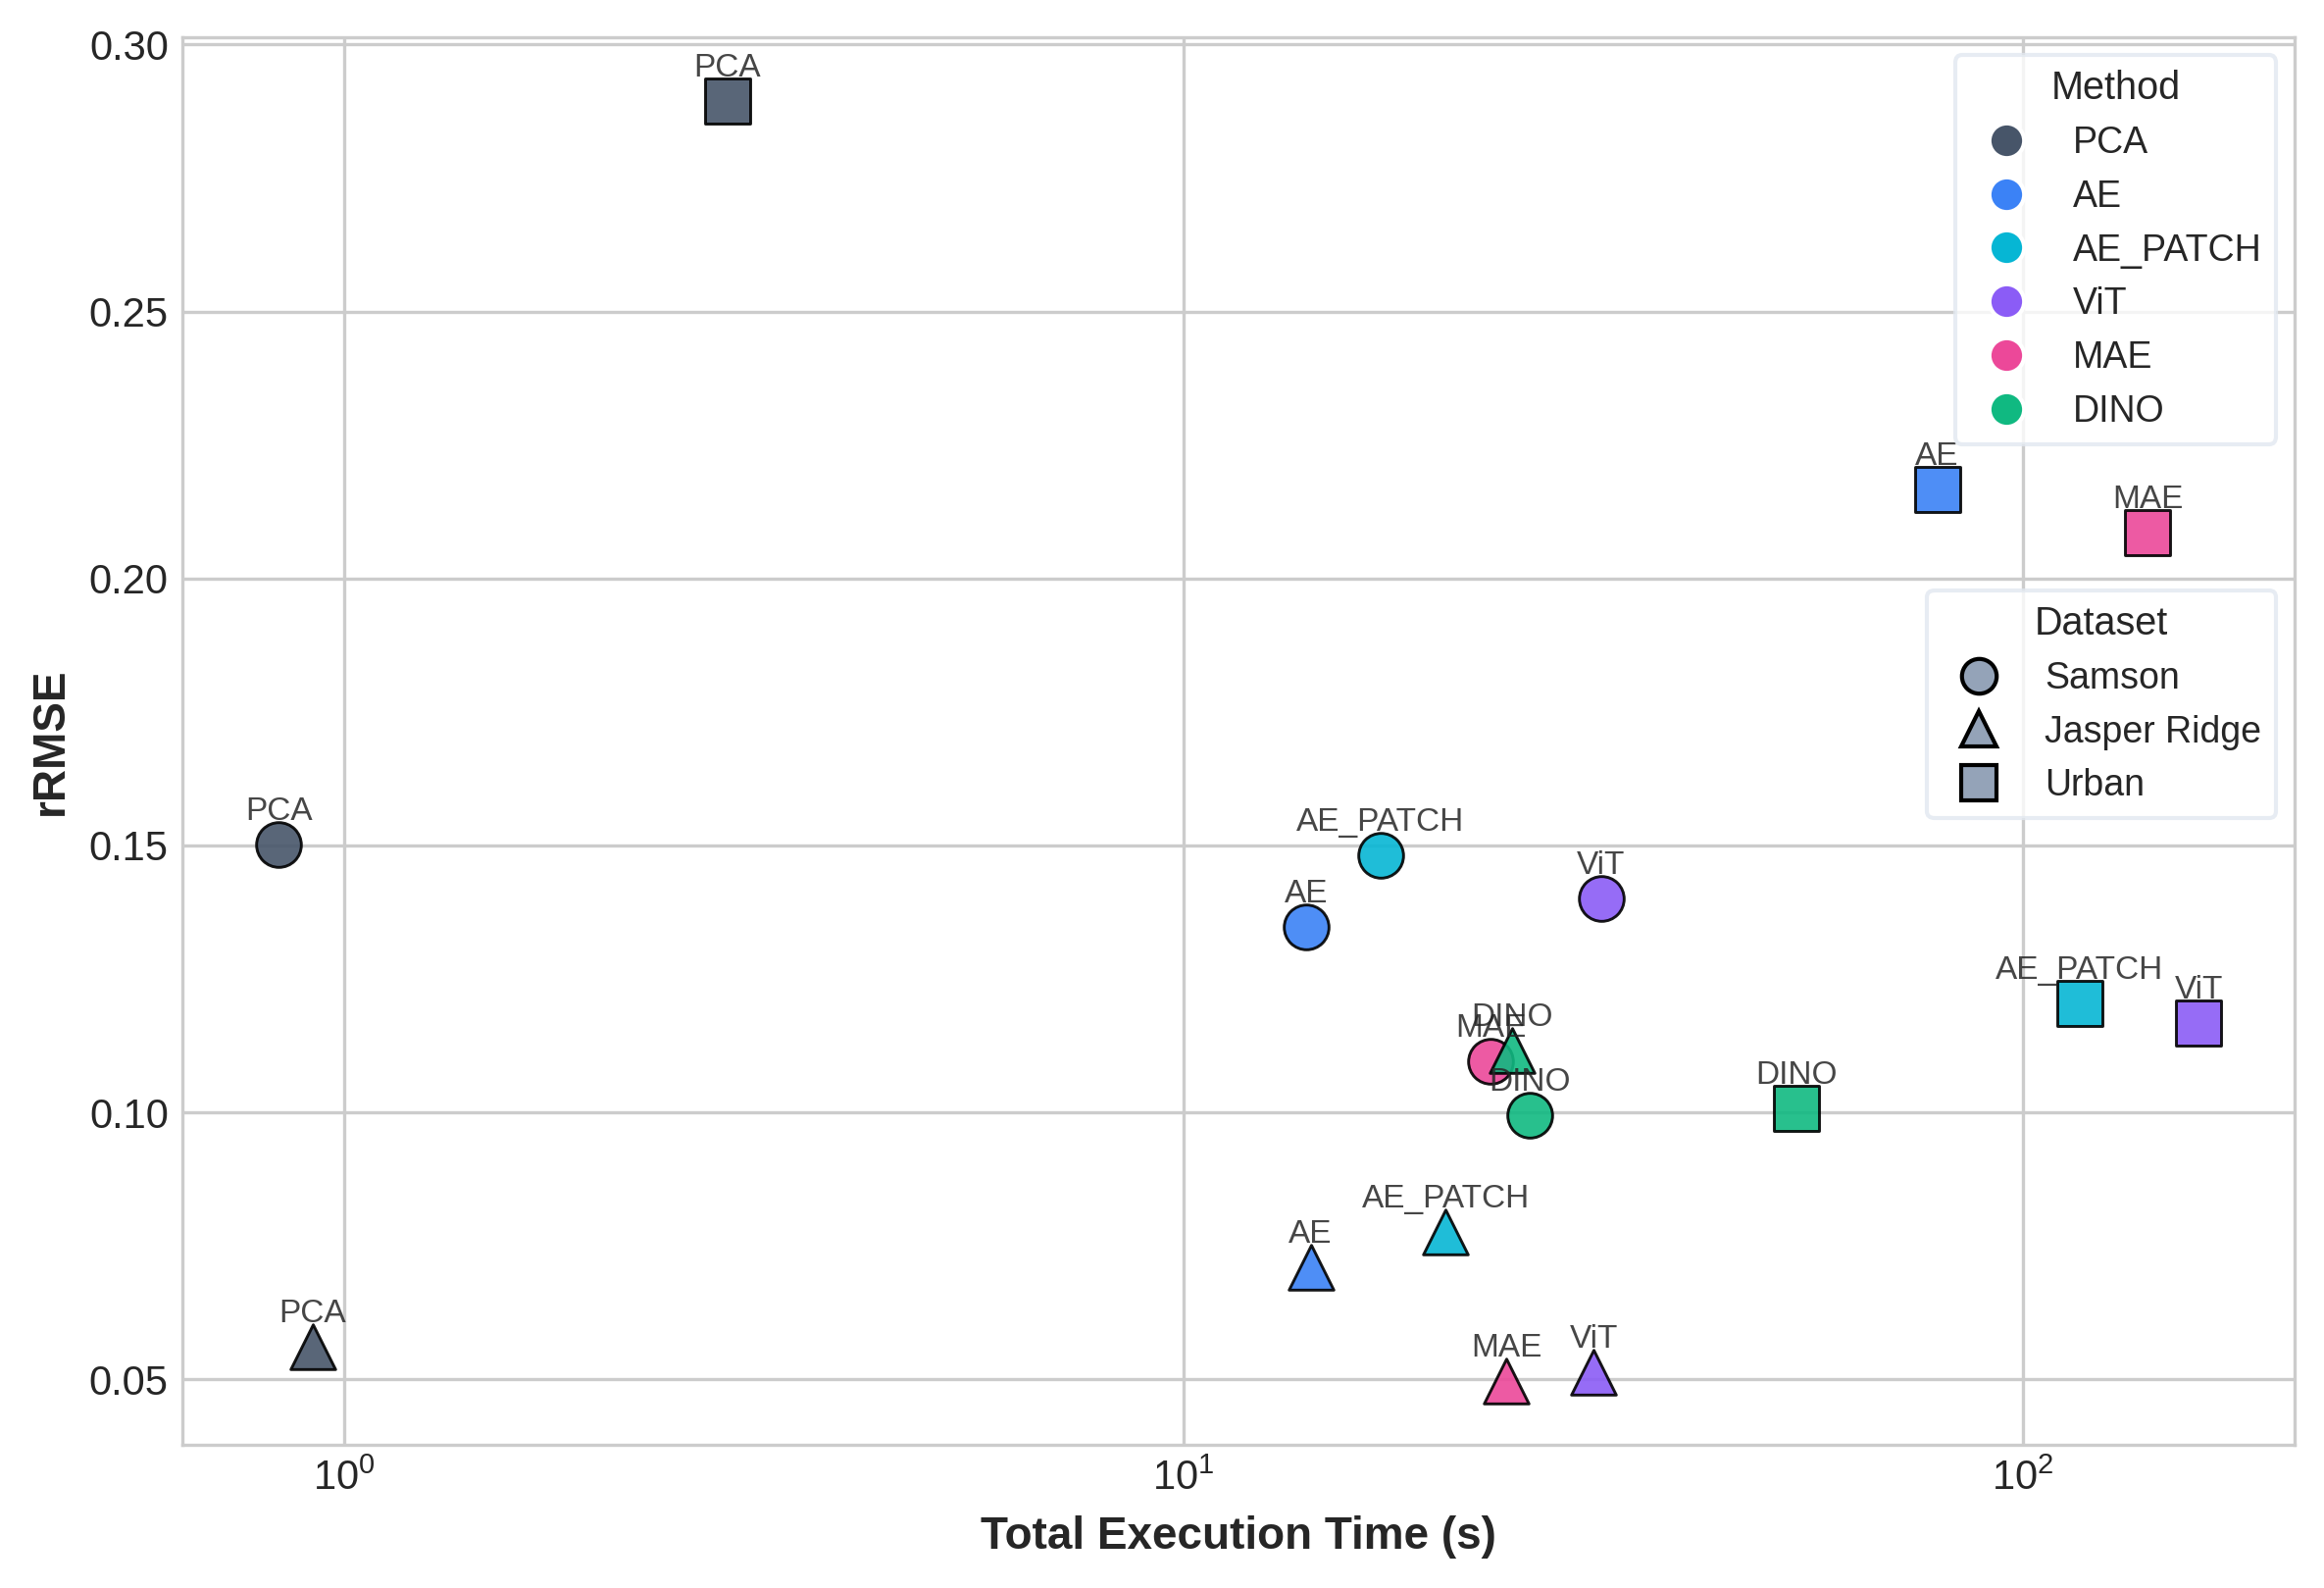
\includegraphics[width=0.80\textwidth]{paper_figures/frontera_eficiencia.png}
    \caption{Multi-metric efficiency frontier: Global accuracy (rRMSE) vs. Total computational time.}
    \label{fig:frontera_eficiencia}
\end{figure}

\subsection{Endmember Spectral Comparison}
\label{subsec:endmember_comparison}

Figures~\ref{fig:endmembers_jasper}--\ref{fig:endmembers_urban} compare the spectral signatures extracted by each dimensionality reduction method with the corresponding ground truth. Jasper Ridge shows larger deviations for Water and Road, whereas Samson exhibits the closest overall agreement. Urban presents the most pronounced discrepancies, particularly for Asphalt, Grass, and Roof, while the Tree signature remains comparatively stable across methods.

\begin{figure}[htbp]
    \centering
    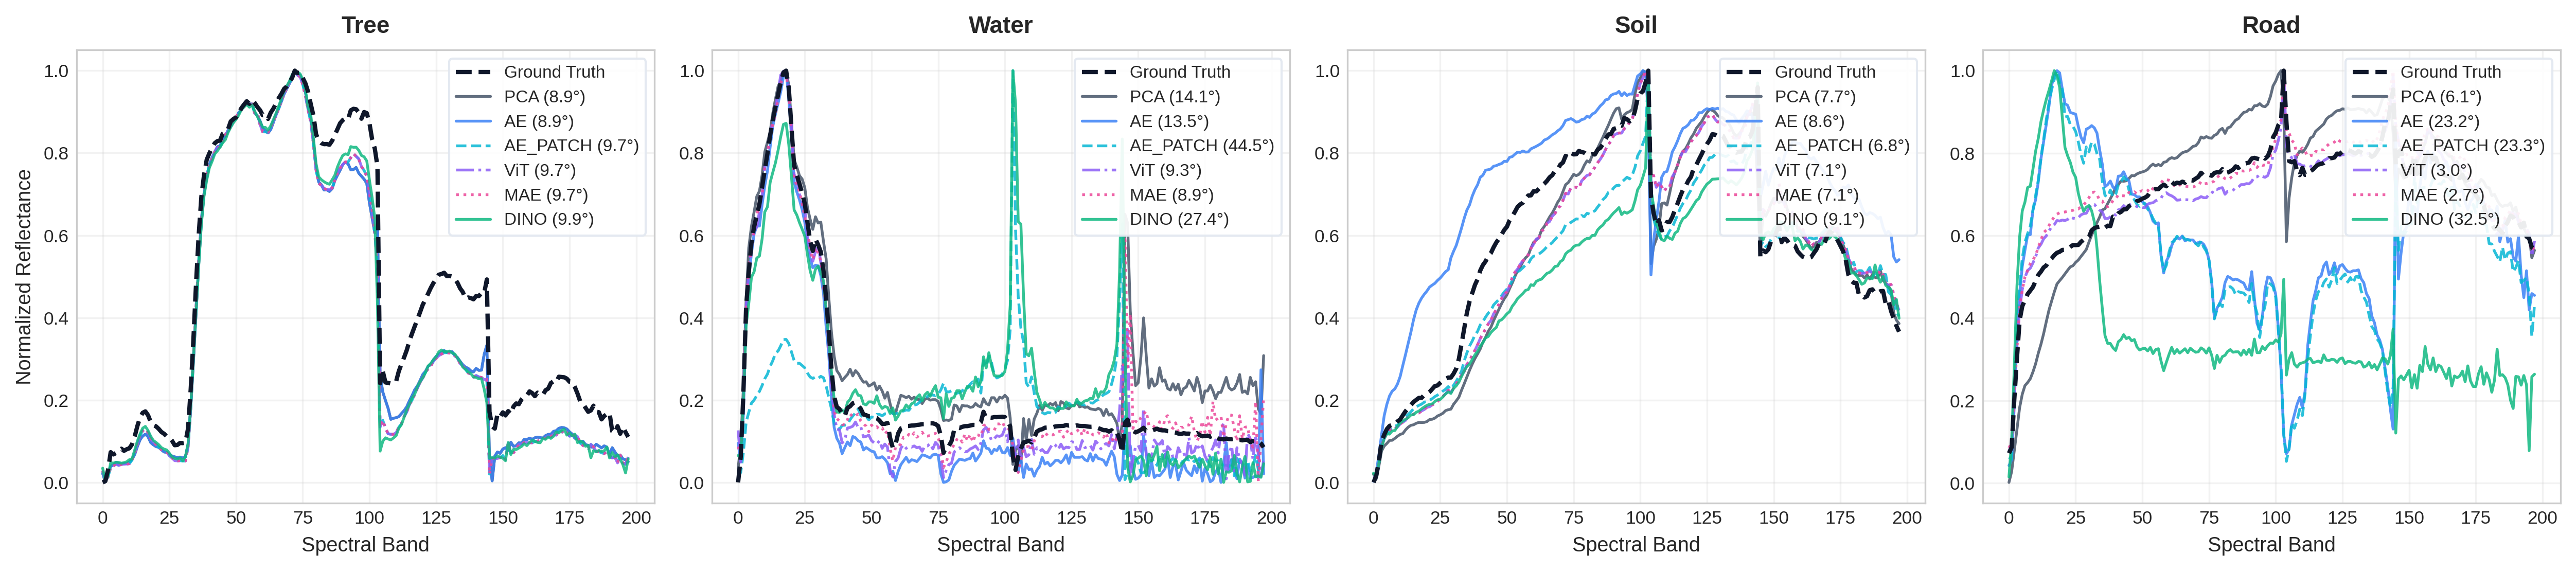
\includegraphics[width=0.98\textwidth]{paper_figures/08_endmembers_vs_gt_jasper.png}
    \caption{Extracted endmember signatures compared with the ground truth for the Jasper Ridge dataset.}
    \label{fig:endmembers_jasper}
\end{figure}

\begin{figure}[htbp]
    \centering
    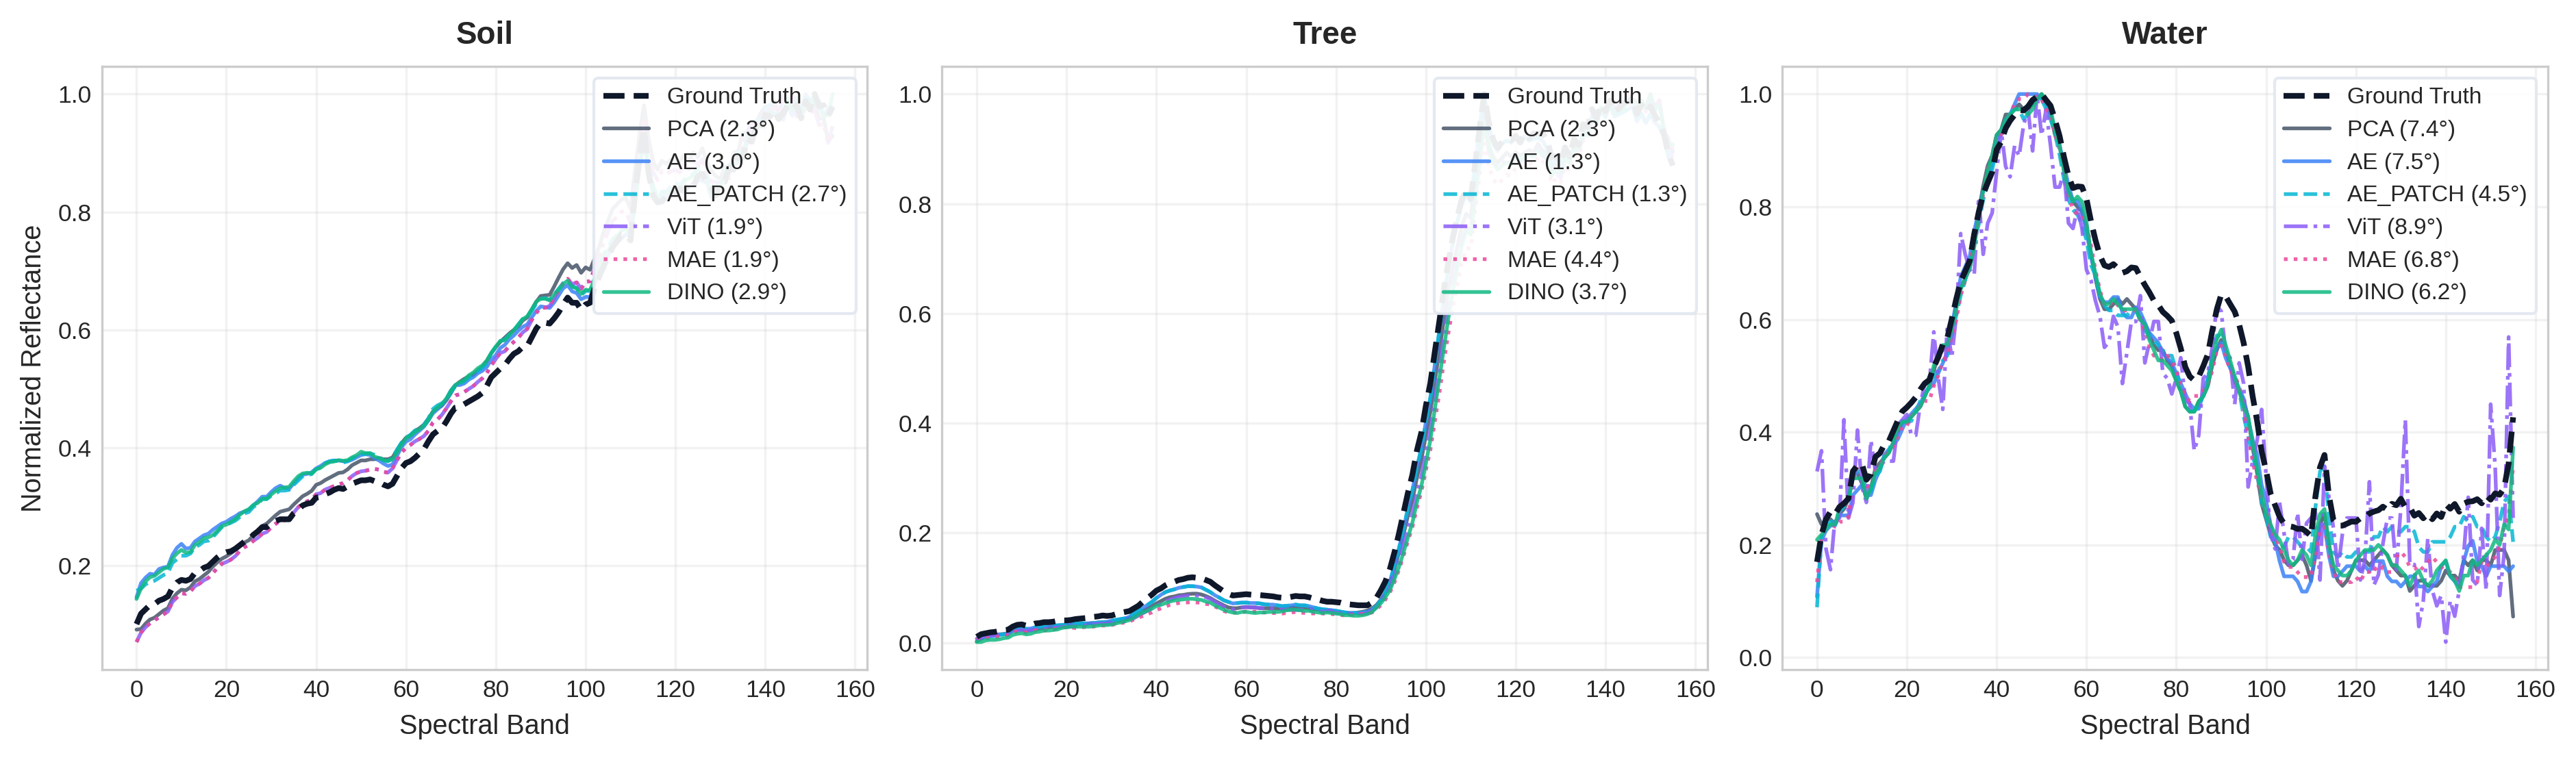
\includegraphics[width=0.98\textwidth]{paper_figures/08_endmembers_vs_gt_samson.png}
    \caption{Extracted endmember signatures compared with the ground truth for the Samson dataset.}
    \label{fig:endmembers_samson}
\end{figure}

\begin{figure}[htbp]
    \centering
    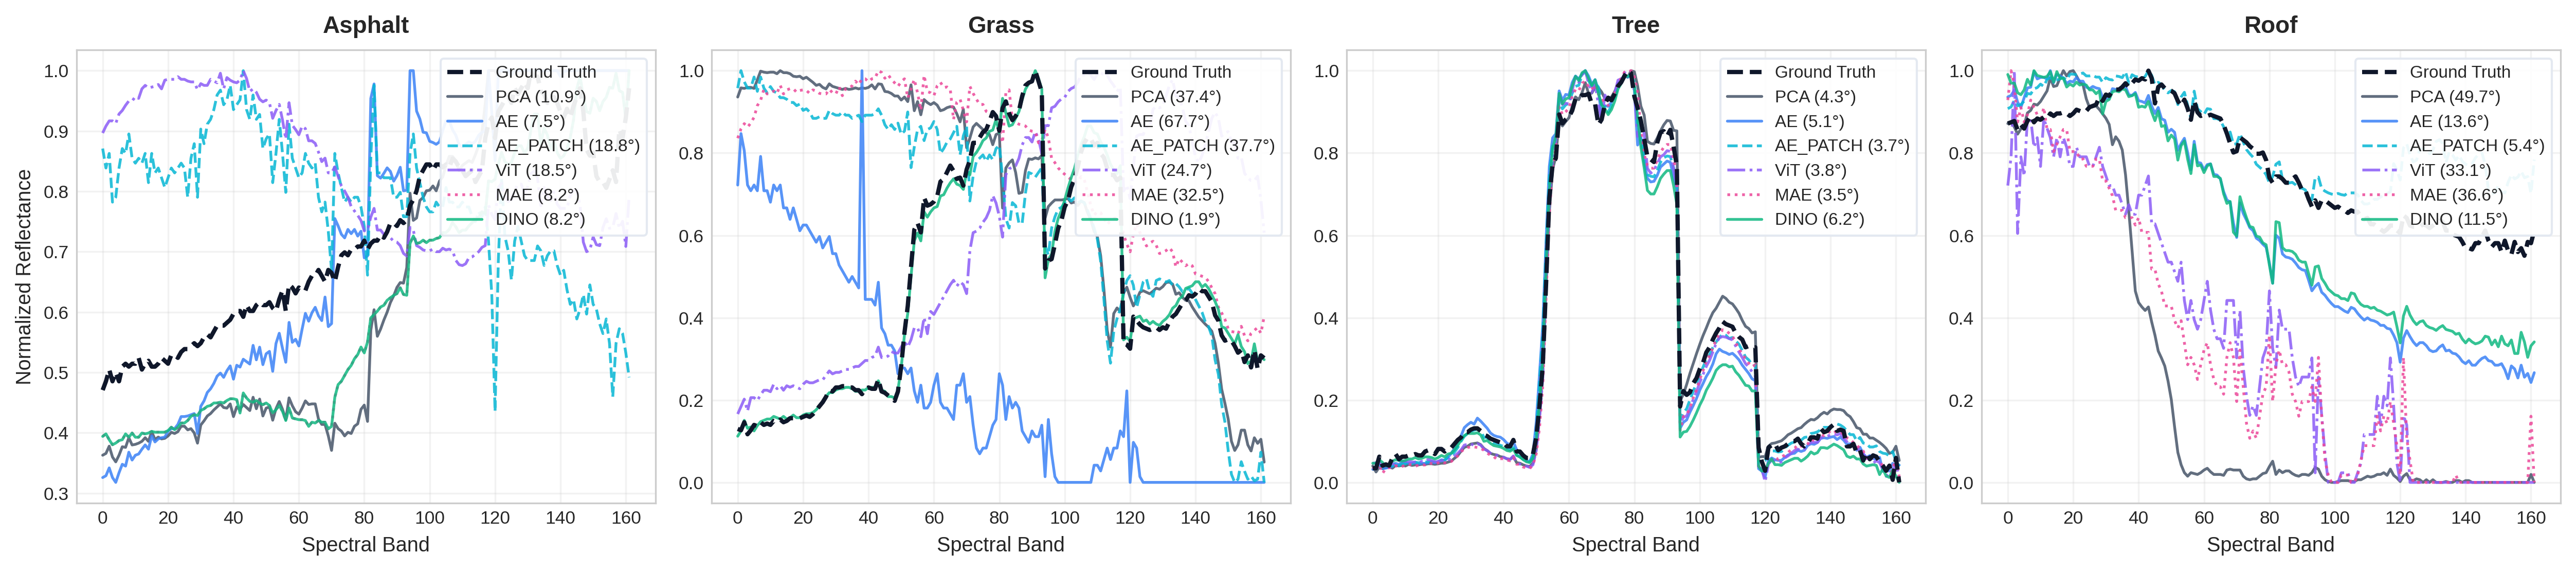
\includegraphics[width=0.98\textwidth]{paper_figures/08_endmembers_vs_gt_urban.png}
    \caption{Extracted endmember signatures compared with the ground truth for the Urban dataset.}
    \label{fig:endmembers_urban}
\end{figure}

The deviations across datasets and materials are consistent with the metric-dependent rankings above: preserving global reconstruction quality does not guarantee that every extracted endmember is aligned with its reference signature. The observed differences do not, by themselves, establish that local spatial context or global attention causes better endmember preservation; isolating those effects would require matched architectures and controlled ablations.

\subsection{Spatial Reconstruction and Error Maps}
\label{subsec:spatial_reconstruction}

To complement the quantitative analysis, Figures~\ref{fig:reconstruction_jasper_ridge}--\ref{fig:reconstruction_urban} present local rRMSE maps that reveal how the reconstruction errors are spatially distributed across the evaluated scenes. These visualizations provide additional insight into the ability of each dimensionality reduction strategy to preserve spatial-spectral structures beyond the global metrics discussed previously.

\begin{figure}[htbp]
    \centering
    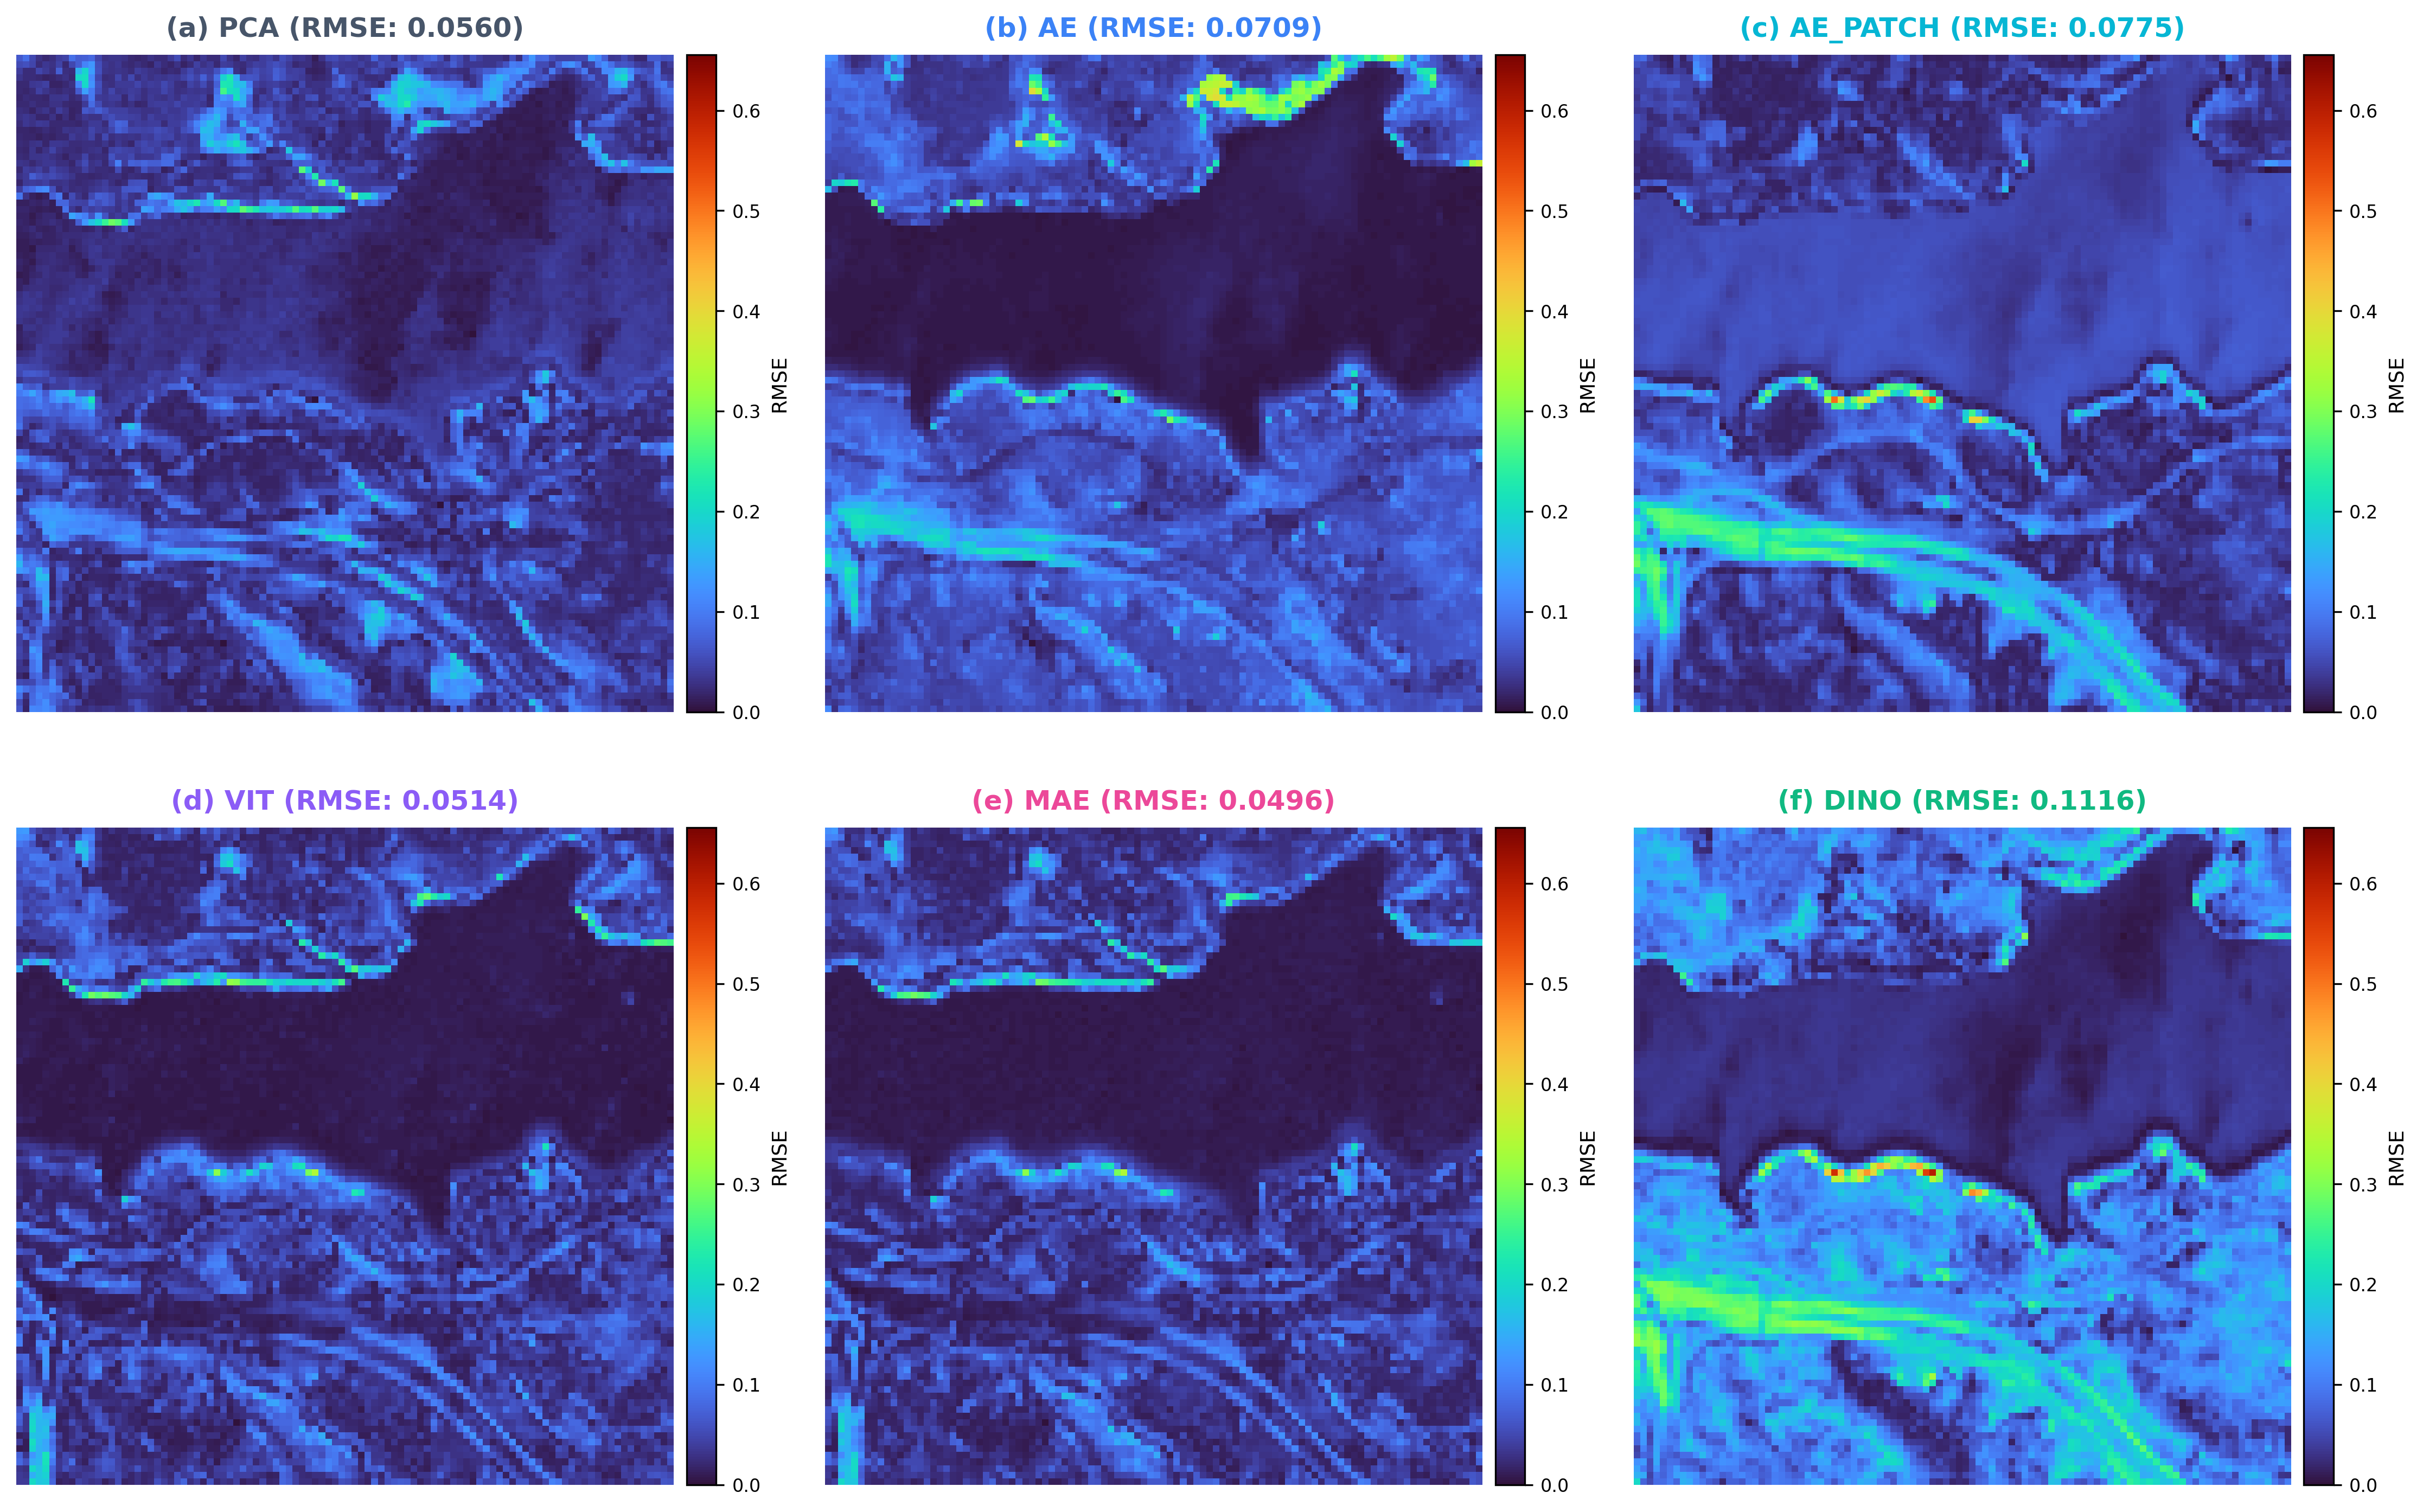
\includegraphics[width=0.98\textwidth]{paper_figures/reconstruccion_jasper_ridge.png}
    \caption{Local rRMSE error maps for the Jasper Ridge dataset.}
    \label{fig:reconstruction_jasper_ridge}
\end{figure}

\begin{figure}[htbp]
    \centering
    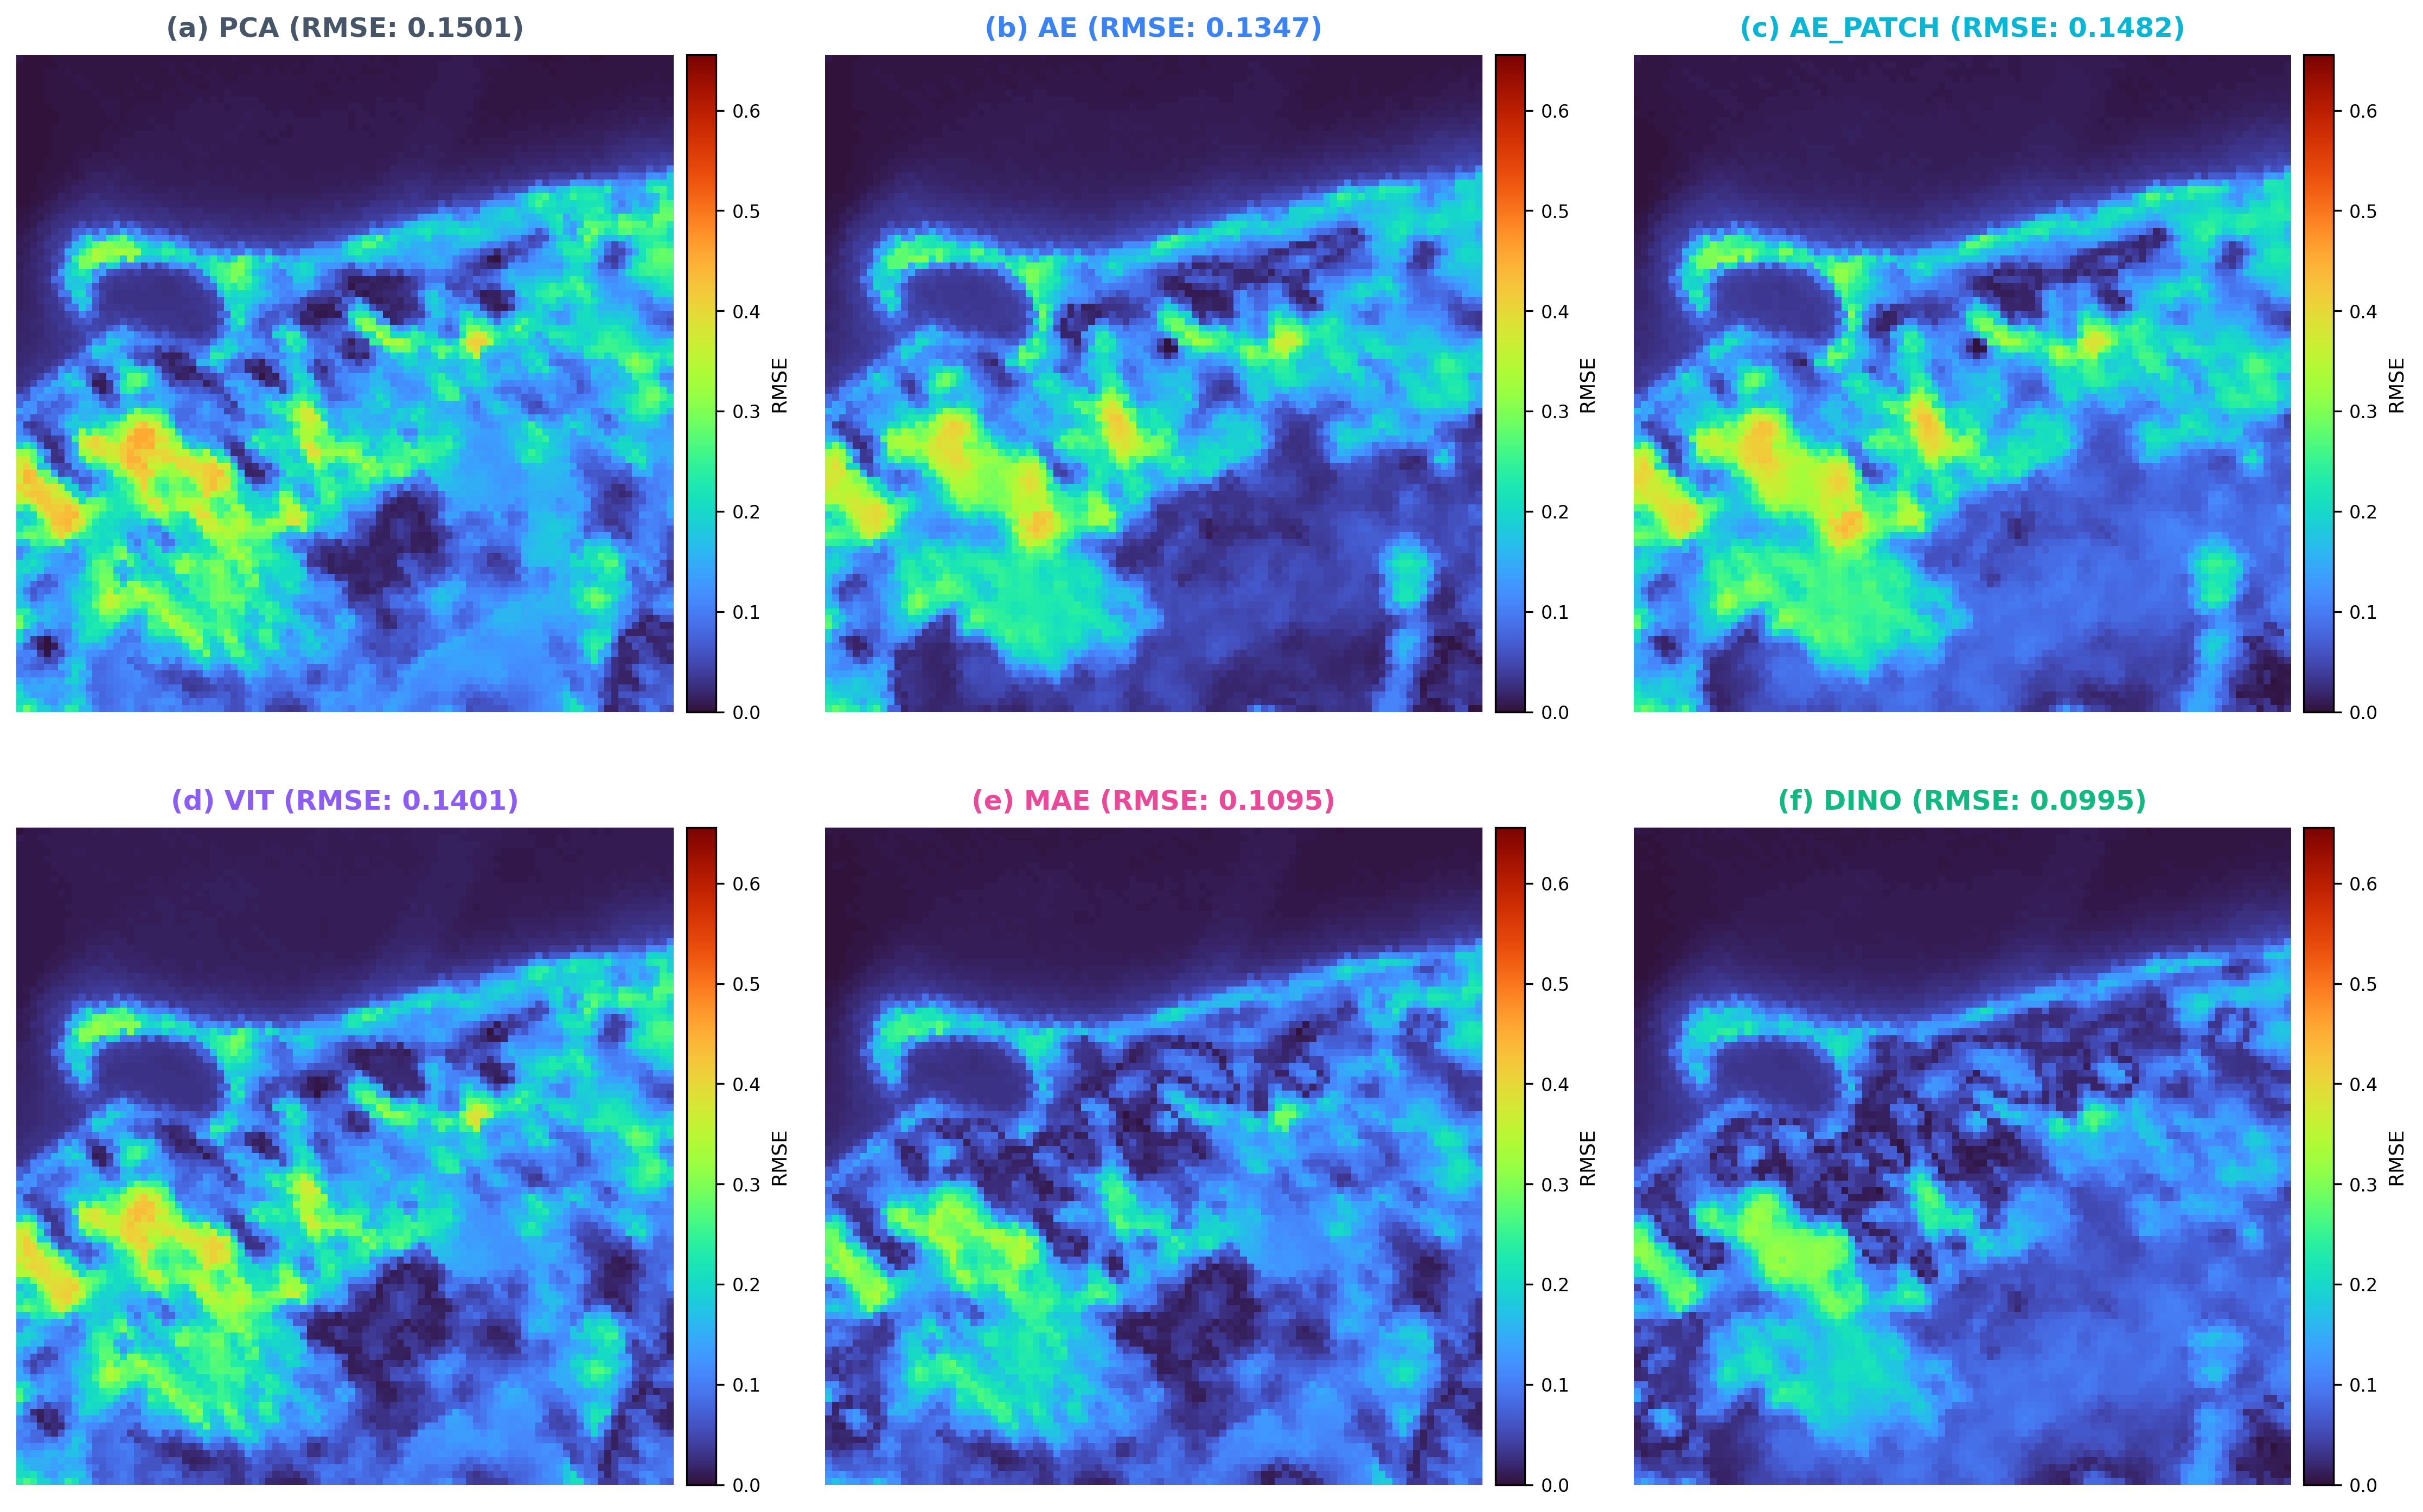
\includegraphics[width=0.98\textwidth]{paper_figures/reconstruccion_samson.png}
    \caption{Local rRMSE error maps for the Samson dataset.}
    \label{fig:reconstruction_samson}
\end{figure}

\begin{figure}[htbp]
    \centering
    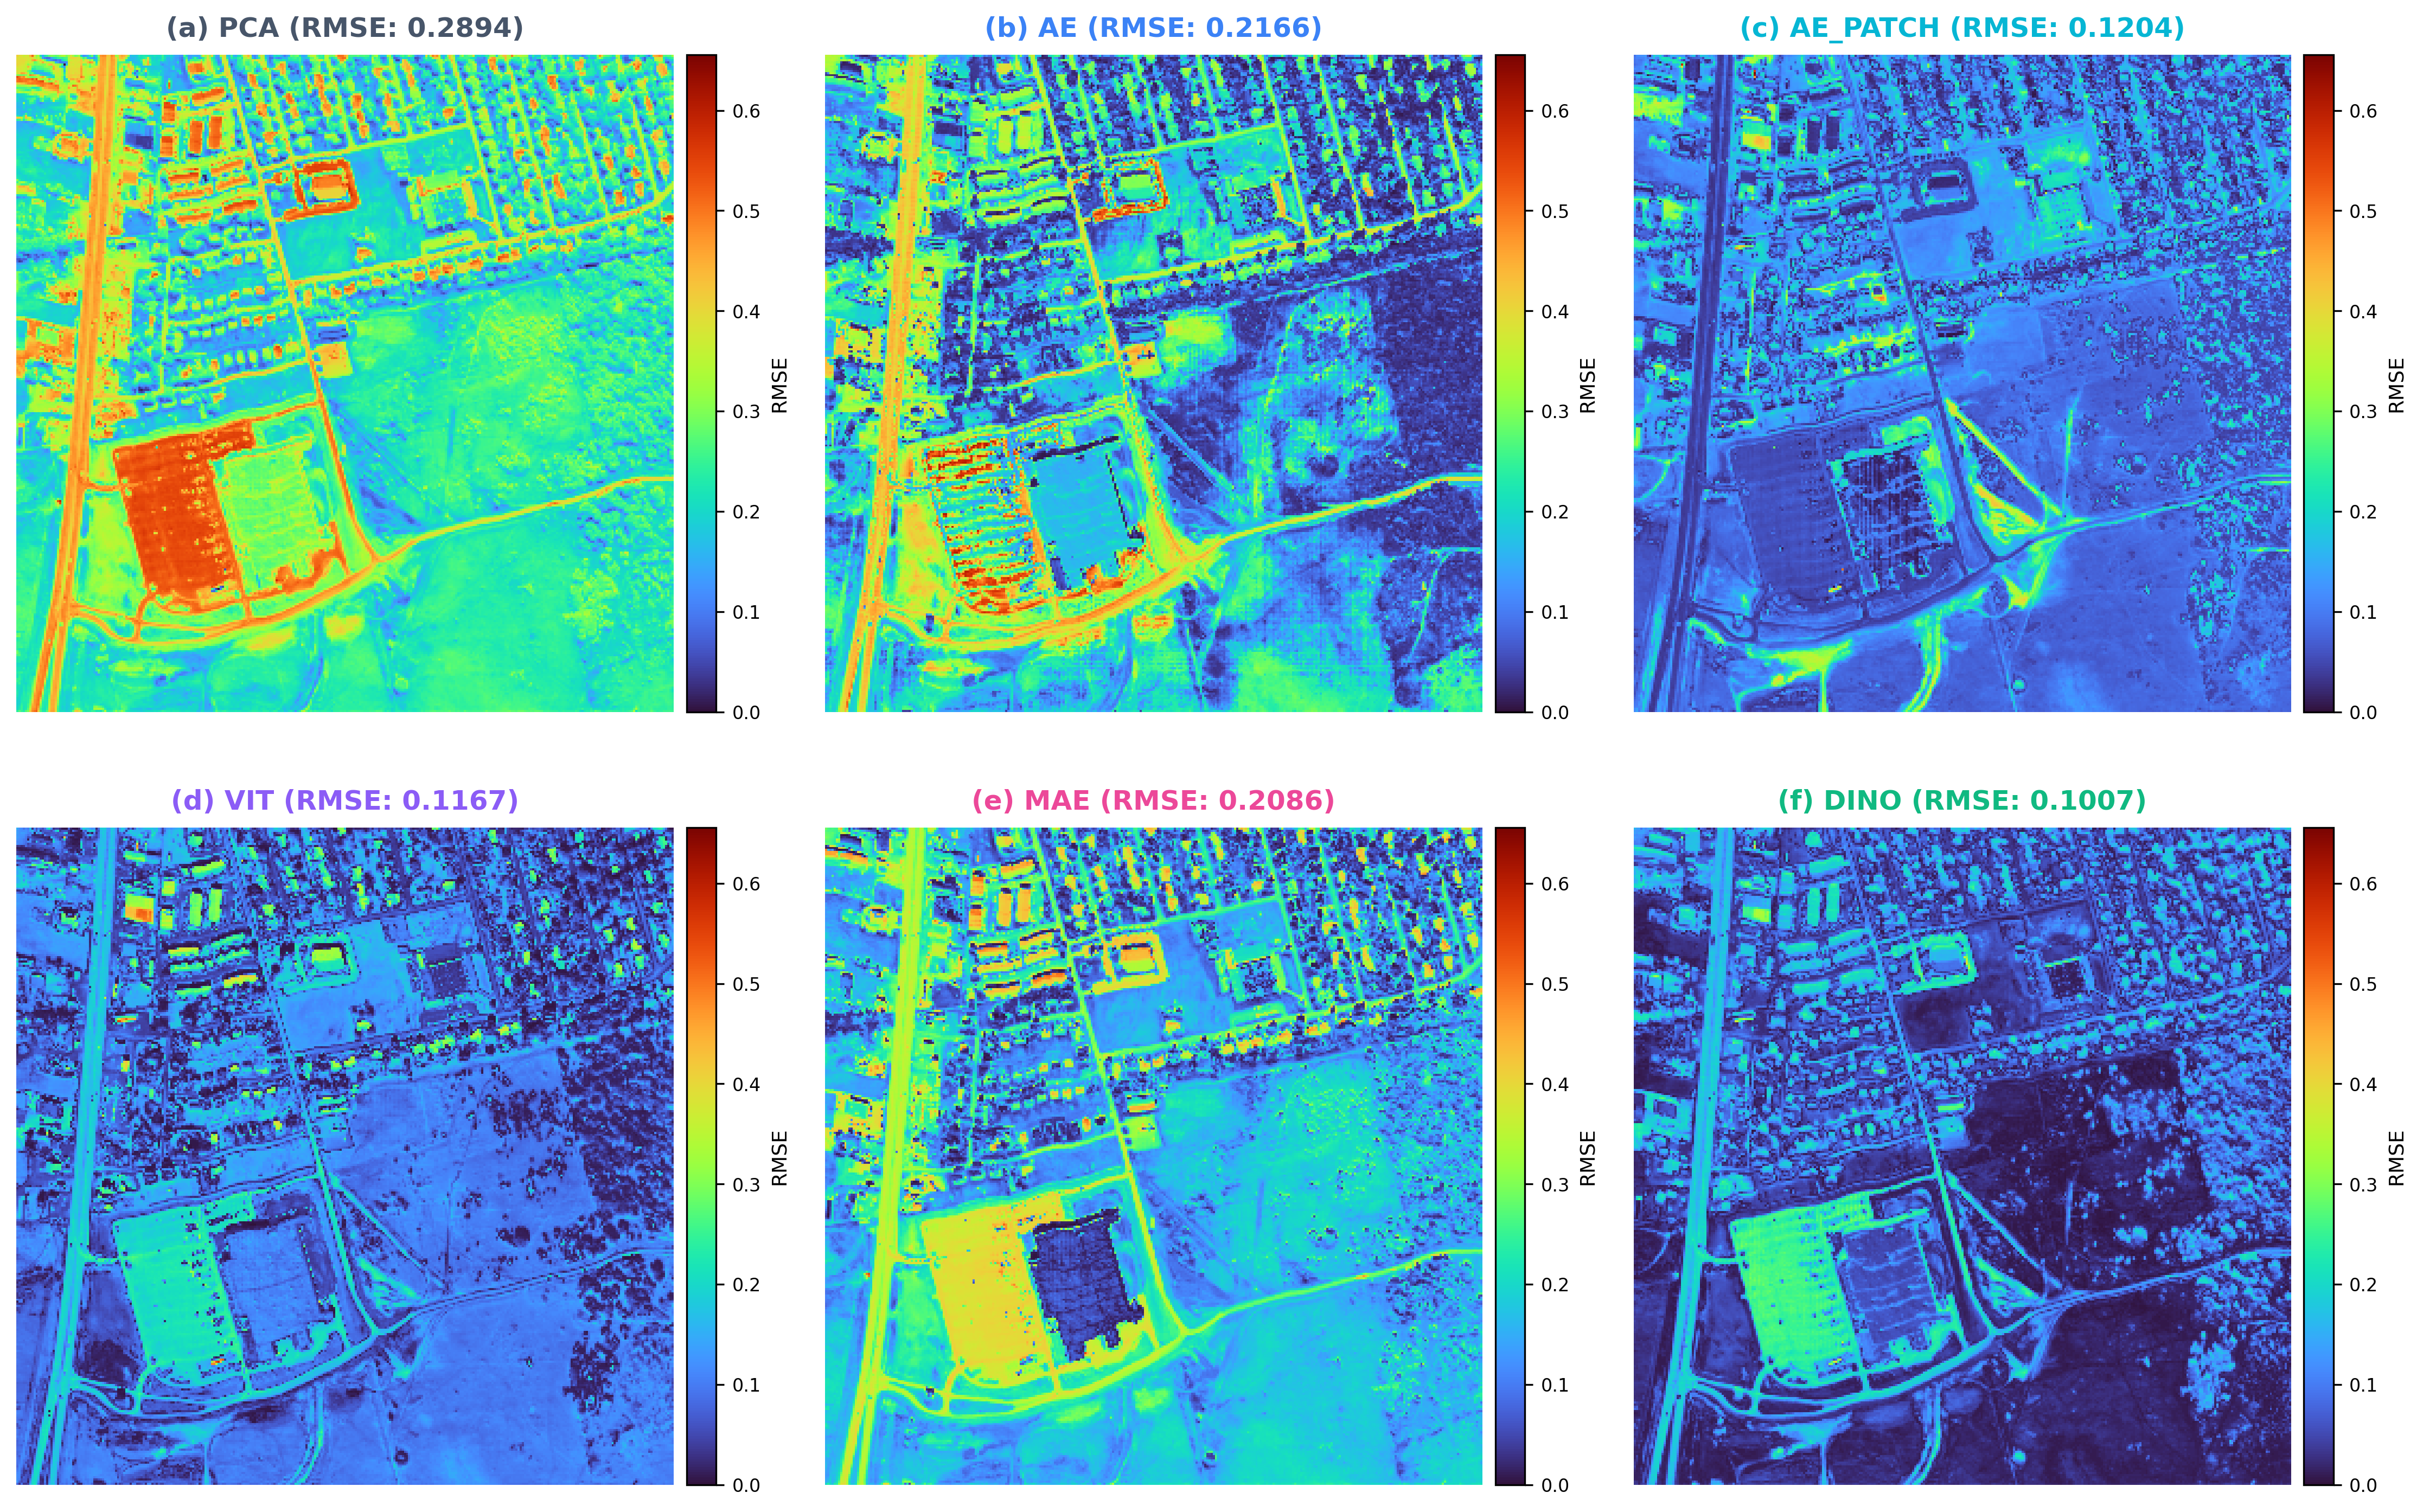
\includegraphics[width=0.98\textwidth]{paper_figures/reconstruccion_urban.png}
    \caption{Local rRMSE error maps for the Urban dataset.}
    \label{fig:reconstruction_urban}
\end{figure}

In Jasper Ridge (Figure~\ref{fig:reconstruction_jasper_ridge}), MAE and ViT produce the most homogeneous error maps, although PCA remains close in global rRMSE and also preserves most regions with low residuals. AE and AE-Patch show stronger errors along boundaries and spatial transitions, while DINO presents the broadest elevation of reconstruction error. Thus, the map does not support a general advantage of deep models over PCA in this dataset; rather, the result depends on the specific learned representation.

In Samson (Figure~\ref{fig:reconstruction_samson}), DINO and MAE reduce the global reconstruction error more effectively than the remaining methods. PCA, AE, AE-Patch, and ViT retain broader regions of moderate error, particularly around spatial transitions and heterogeneous or shadowed areas. The persistence of these localized residuals despite the presence of only three reference classes indicates that scene illumination and pixel mixing remain important sources of difficulty.

Urban (Figure~\ref{fig:reconstruction_urban}) exhibits the largest separation among methods. PCA produces widespread high residuals, while AE and MAE retain substantial error over infrastructure and transition regions. AE-Patch and ViT reduce these errors considerably, and DINO provides the lowest and most spatially uniform residual distribution, consistent with its rRMSE of 0.1007. The weak Urban result of MAE also confirms that the transformer-based methods do not improve uniformly under highly mixed conditions. Determining which architectural or training component produces these differences would require controlled ablations.

Taken together, the spatial maps provide qualitative context for the decoupling between reconstruction, endmember, and abundance metrics. Jasper Ridge shows relatively low reconstruction error for several methods even when extracted endmembers differ from their references. Samson retains localized errors in shadowed and mixed transition regions, while Urban combines spectrally similar vegetation, strongly mixed pixels, and within-class variability in materials such as roofs and asphalt. Thus, low residuals in selected regions do not necessarily imply reliable abundance estimates. These interpretations are based on visual patterns and should be tested with stratified analyses of shadow, mixture, and within-class variability; they do not establish representation collapse or identify a specific loss function as inadequate.

\section{Discussion}
\label{sec:discussion}

% Include from the project root; requires graphicx.
\begin{figure*}[t]
    \centering
    \includegraphics[width=0.98\textwidth]{in_deep_analysis/fig_spatial_error_analysis.png}
    \caption{Selected spatial reconstruction comparisons for (a) Samson, (b) Jasper Ridge,
    and (c) Urban. Columns show the full pseudo-RGB scene and ROI, the dominant
    ground-truth material in the ROI, the competing system, and DINO. Error maps
    show pixelwise reconstruction RMSE (rRMSE). Each pair shares the same color
    limits within its row; limits may differ between rows. Annotations report
    ROI rRMSE, computed as the root mean square of the pixelwise errors.
    The prefix $r$ denotes reconstruction, not relative normalization.}
    \label{fig:spatial_error_analysis}
\end{figure*}

\subsection{Spatial Error Localization}
\label{subsec:spatial_error_tradeoffs}

Column~3 uses PCA for Samson and Urban as the conventional linear reference.
MAE is used for Jasper Ridge because it has the lowest global reconstruction
rRMSE among the evaluated systems in that scene. These selected comparisons
illustrate spatial differences; they do not isolate architectural or training
mechanisms, and do not establish a ranking of all systems within each ROI.

In Samson, the selected shoreline, canopy, and soil ROI has
rRMSE of $0.170$ for PCA and $0.112$ for DINO, a $34.1\%$ reduction. In Jasper
Ridge, MAE has lower ROI rRMSE than DINO ($0.042$ versus $0.095$),
while DINO reaches a maximum pixelwise rRMSE of $0.602$ in this ROI. The
matched Road endmember also differs substantially: its SAD is $2.71^\circ$
for MAE and $32.45^\circ$ for DINO. In the selected Urban ROI, DINO has
rRMSE of $0.122$, compared with $0.324$ for PCA, a $62.2\%$ reduction.
The same rRMSE formula is used for ROIs and full cubes; their values may
differ because they evaluate different sets of pixels.

The transformer inputs use $3\times3$ spatial neighborhoods. DINO's student
also receives center-token occlusion during training and uses a learned CLS
representation. These design choices motivate hypotheses about sensitivity
to local context, but the maps alone cannot demonstrate that the CLS token
averages road spectra, that road pixels cease to be latent extreme points,
or that self-distillation causes the observed errors. The results support a
scene- and material-dependent comparison, consistent with the separate
local--global summary, rather than a universal advantage for any architecture.

% Include from the project root; requires \usepackage{graphicx}.
% % Include from the project root; requires \usepackage{graphicx}.
% % Include from the project root; requires \usepackage{graphicx}.
% \input{local_global/local_global_summary.tex}
\begin{figure}[htbp]
    \centering
    \includegraphics[width=\linewidth]{local_global/local_global_summary.png}
    \caption{Agreement between global reconstruction, local reconstruction, and endmember fidelity.
    Bar labels report matching regions out of all material regions; each region comprises
    pixels sharing the dominant ground-truth material. The right column identifies the
    method with the lowest mean endmember SAD.}
    \label{fig:local_global_summary}
\end{figure}

Figure~\ref{fig:local_global_summary} contrasts scene-level reconstruction with material-level preservation. The fractions of material regions where the global RMSE winner also minimizes local RMSE are 1/3 in Samson, 1/4 in Jasper Ridge, and 2/4 in Urban. In Samson, AE-Patch has the lowest mean endmember SAD, despite DINO achieving the lowest global RMSE. Thus, global reconstruction quality alone does not establish uniform preservation of every material region and endmember.

\begin{figure}[htbp]
    \centering
    \includegraphics[width=\linewidth]{local_global/local_global_summary.png}
    \caption{Agreement between global reconstruction, local reconstruction, and endmember fidelity.
    Bar labels report matching regions out of all material regions; each region comprises
    pixels sharing the dominant ground-truth material. The right column identifies the
    method with the lowest mean endmember SAD.}
    \label{fig:local_global_summary}
\end{figure}

Figure~\ref{fig:local_global_summary} contrasts scene-level reconstruction with material-level preservation. The fractions of material regions where the global RMSE winner also minimizes local RMSE are 1/3 in Samson, 1/4 in Jasper Ridge, and 2/4 in Urban. In Samson, AE-Patch has the lowest mean endmember SAD, despite DINO achieving the lowest global RMSE. Thus, global reconstruction quality alone does not establish uniform preservation of every material region and endmember.

\begin{figure}[htbp]
    \centering
    \includegraphics[width=\linewidth]{local_global/local_global_summary.png}
    \caption{Agreement between global reconstruction, local reconstruction, and endmember fidelity.
    Bar labels report matching regions out of all material regions; each region comprises
    pixels sharing the dominant ground-truth material. The right column identifies the
    method with the lowest mean endmember SAD.}
    \label{fig:local_global_summary}
\end{figure}

Figure~\ref{fig:local_global_summary} contrasts scene-level reconstruction with material-level preservation. The fractions of material regions where the global RMSE winner also minimizes local RMSE are 1/3 in Samson, 1/4 in Jasper Ridge, and 2/4 in Urban. In Samson, AE-Patch has the lowest mean endmember SAD, despite DINO achieving the lowest global RMSE. Thus, global reconstruction quality alone does not establish uniform preservation of every material region and endmember.


\section{Conclusions}
\label{sec:conclusions}

This work evaluated six dimensionality reduction methods (PCA, AE, AE-Patch, ViT, MAE, and DINO) within a fixed linear spectral unmixing pipeline based on N-FINDR and FCLSU, using the Samson, Jasper Ridge, and Urban datasets. The results do not identify a universally superior method: reconstruction, endmember fidelity, abundance accuracy, and computational cost vary with both dataset and evaluation metric. For example, DINO leads the reported reconstruction and unmixing metrics in Urban, but performs less favorably in Jasper Ridge; AE-Patch yields the lowest mSAD in Samson, while MAE and ViT lead selected metrics in Jasper Ridge. These findings do not support a general claim that transformer-based methods consistently outperform the alternatives.

Method selection should therefore reflect the target scene, the fidelity criterion required by the application, and the available computational budget. Because this study evaluates only a linear unmixing workflow, its rankings should not be assumed to generalize to nonlinear mixing conditions or other downstream tasks. Future work should compare reference and reconstructed endmember signatures directly, conduct stratified analyses of shadowed and mixed regions, and use controlled ablations to test architectural and training choices. Evaluations with nonlinear unmixing models and additional downstream tasks would further establish the scope of these findings.




\section*{Acknowledgments}
Anyone who made a contribution to the research or manuscript, but who is not a listed author, should be acknowledged (with their permission). Types of acknowledgements include:

\subsection*{General}
Thank others for any contributions, whether it be direct technical help or indirect assistance

\subsection*{Author Contributions}
Describe contributions of each author to the paper, using the first initial and full last name.

\medskip Examples:

``S. Zhang conceived the idea and designed the experiments.''

``E. F. Mustermann and J. F. Smith conducted the experiments.''

``All authors contributed equally to the writing of the manuscript.''

\subsection*{Funding}
Name financially supporting bodies (written out in full), followed by the funding awardee and associated grant numbers (if applicable) in square brackets.

\medskip Example:

``This work was supported by the Engineering and Physical Sciences Research Council [grant numbers xxxx, yyyy]; the National Science Foundation [grant number zzzz]; and a Leverhulme Trust Research Project Grant.''

\medskip
If the research did not receive specific funding, but was performed as part of the employment of the authors, please name this employer. If the funder was involved in the manuscript writing, editing, approval, or decision to publish, please declare this.

\subsection*{Conflicts of Interest}
Conflicts of interest (COIs, also known as ``competing interests'') occur when issues outside research could be reasonably perceived to affect the neutrality or objectivity of the work or its assessment.

Authors must declare all potential interests – whether or not they actually had an influence – in a ‘Conflicts of Interest’ section, which should explain why the interest may be a conflict. Authors must declare current or recent funding (including for Article Processing Charges) and other payments, goods or services that might influence the work. All funding, whether a conflict or not, must be declared in a ``Funding Statement.'' The involvement of anyone other than the authors who 1) has an interest in the outcome of the work; 2) is affiliated to an organization with such an interest; or 3) was employed or paid by a funder, in the commissioning, conception, planning, design, conduct, or analysis of the work, the preparation or editing of the manuscript, or the decision to publish must be declared.

If there are none, the authors should state ``The author(s) declare(s) that there is no conflict of interest regarding the publication of this article.'' Submitting authors are responsible for coauthors declaring their interests. Declared conflicts of interest will be considered by the editor and reviewers and included in the published article.

\subsection*{Data Availability}
A data availability statement is compulsory for all research articles. This statement describes whether and how others can access the data supporting the findings of the paper, including 1) what the nature of the data is, 2) where the data can be accessed, and 3) any restrictions on data access and why.

If data are in an archive, include the accession number or a placeholder for it. Also include any materials that must be obtained through a Material Transfer Agreements (MTA).

\section*{Supplementary Materials}
Describe any supplementary materials submitted with the manuscript (e.g., audio files, video clips or datasets).

Please group supplementary materials in the following order: materials and methods, figures, tables, and other files (such as movies, data, interactive images, or database files).

\medskip Example:
Fig. S1. Title of the first supplementary figure.

Fig. S2. Title of the second supplementary figure.

Table S1. Title of the first supplementary table.

Data file S1. Title of the first supplementary data file.

Movie S1. Title of the first supplementary movie.

\medskip
Be sure to submit all supplementary materials with the manuscript and remember to reference the supplementary materials at appropriate points within the manuscript. We recommend citing specific items, rather than referring to the supplementary materials in general, for example: ``See Figures S1-S10 in the Supplementary Material for comprehensive image analysis.''

A link to access the supplementary materials will be provided in the published article.

Supplementary Materials may include additional author notes—for example, a list of group authors.

\section*{Guidelines for References}

There is only one reference list for all sources cited in the main text, figure and table legends, and Supplementary Materials. Do not include a second reference list in the Supplementary Materials section. Include references cited only in the Supplementary Materials at the end of the reference section of the main text; reference numbering should continue as if the Supplementary Materials are a continuation of the main text. References cited only in the Supplementary Materials section are not counted toward length guidelines.

Authors are responsible for ensuring that the information in each reference is complete and accurate.

DOIs, if available, should be included for each reference.

Please do not include any extraneous language such as explanatory notes as part of a reference to a given source. The Journal of Remote Sensing prefers that manuscripts do not include end notes; if information is important enough to include, please put into main text.  If you need to include notes, please explain why they are needed in your cover letter to the editor.

\printbibliography

\end{document}
